\documentclass[11pt,twocolumn,notitlepage,openany,twoside]{book}
\usepackage[paperheight=11.25in,paperwidth=8.75in, margin=0.625in]{geometry}
\usepackage{titlesec}
\usepackage{verbatim}
\pagestyle{headings}

% Figure setup
\usepackage[]{graphicx}
\graphicspath{ {figures/} }
\usepackage{float}
%\setlength{\floatsep}{0pt plus 2.0pt minus 2.0pt}
%\setlength{\dbltextfloatsep}{5pt plus 2.0pt minus 2.0pt}
\usepackage{caption}
\captionsetup[figure]{font=small}

% For supplemental figure labeling
\usepackage{newfloat}
\DeclareFloatingEnvironment[name={Supplemental Figure}]{suppfigure}


% Remove the giant space at the beginning of a chapter
\titleformat{\chapter}[display]
    {\normalfont\huge\bfseries}{\chaptertitlename\ \thechapter}{20pt}{\Huge}
\titlespacing*{\chapter}{0pt}{0pt}{20pt}

\title{Metabolic interactions and capabilities within microbial communities}
\author{Gregory Leonard Medlock}


% Optimization problem formatting
\usepackage{amsmath}

% Needed for \textmu in text for microliters
\usepackage{textcomp}

% needed for other greek characters in text
\usepackage{textgreek}

% non-optimization algorithm formatting
\usepackage{algorithm}% http://ctan.org/pkg/algorithm
\usepackage[noend]{algpseudocode}


%
% % Bibliography setup
% \usepackage[backend=biber, style=numeric-comp,sorting=none,terseinits=true, giveninits=true,maxbibnames=4]{biblatex}
% \addbibresource{rf_references.bib}
% \DeclareNameAlias{default}{last-first}
% \renewcommand*{\revsdnamepunct}{}
% \renewcommand*{\bibfont}{\small}

\usepackage[backend=biber, style=numeric-comp,sorting=none,terseinits=true, giveninits=true,maxbibnames=4]{biblatex}
\addbibresource{rf_compiled_refs.bib}
%\renewcommand*{\bibfont}{\small}


% There's a non-ASCII character somewhere in the bib, so we need this package:
\usepackage[utf8]{inputenc}

\begin{document}
\frontmatter

\clearpage
% Cover page
\begin{titlepage}
   \begin{center}
       \vspace*{1cm}

       \LARGE
       \textbf{Metabolic interactions and capabilities within microbial communities}


       \vspace{1.5cm}

       \Large
       By\\
       \textbf{Gregory L. Medlock}

       \vspace{2.5cm}

       A dissertation presented to the faculty of the School of Engineering and Applied Science in partial fulfillment of the requirements for the degree of\\

       \vspace{1.5cm}

       Doctor of Philosophy

       \vspace{1.5cm}

       Department of Biomedical Engineering\\
       University of Virginia\\
       Charlottesville, Virginia\\
       May, 2019

   \end{center}
\end{titlepage}

\clearpage
This page intentionally left blank for signed approval sheet.
\clearpage

\begingroup
\let\clearpage


\setcounter{tocdepth}{3}
\tableofcontents
\hspace{1.5cm}
\listoffigures
\hspace{1.5cm}


\endgroup
\clearpage
\addcontentsline{toc}{chapter}{Acknowledgments}
\section{Acknowledgments}
\thispagestyle{plain}
Graduate school has been the most challenging yet fulfilling phase of my life so far. My experience was overwhelmingly shaped by the people and environment at the University of Virginia and the Charlottesville area.

My path to UVA was serendipitous---as an undergraduate at the University of Washington, I felt confident that I wanted to pursue a career in research, so I knew that I would need a PhD. I count myself very lucky for having applied to and chosen UVA. The main reason I applied to UVA was that a friend and mentor one class ahead of me at the UW, Jacqueline Robinson-Hamm, mentioned that the UVA faculty were incredibly personable during her interviews. UVA BME had faculty in systems biology whose research interested me, so I gave it a shot. Over the years that followed, I learned just how accurate Jacqueline's impression of the faculty was, and am incredibly thankful for her tip.

I thank my advisor, Jason Papin, for taking a chance on me and providing an environment for me to grow the scientist in myself. As I mature professionally and look back on my experiences, I am constantly in awe of Jason's patience, humility, and deliberate investment in mentorship. I also thank my doctoral committee members, who each have been fully committed to my personal and professional development as a scientist since the very first day we met. I also thank all of the faculty members at UVA and abroad who have informally mentored me, including Richard Guerrant and Jonathan Swann.

My wife, Maureen Carey, has been an unwavering source of support, motivation, and fun throughout our time in Charlottesville. Her indomitable passion for building a career that impacts the lives of others, both through science itself and the relationships she builds along the way, constantly reminds me of the good in humanity. Maureen's thoughtfulness touches all of her relationships, and I am lucky enough to experience this both personally and professionally. I thank her for making the work in this dissertation possible and letting me see the world through her eyes. I am also forever indebted to Charlottesville for bringing the two of us together.

I thank my siblings Scott, Cami, Brad, Donnie, and Vicki, for a childhood full of joy and for the role models they have all been throughout my life. Growing up in a large family can be chaotic, but it also provides a sense of comradery that no other relationship can replace. I thank the smart, creative, and caring friends I met throughout grade school in Puyallup and during my time at the University of Washington. I am grateful for friends that helped me make it through the UW bioengineering curriculum-induced late nights---especially Jacqueline, Ross Jones, and Hunter Bennett. I thank my lifelong friend and best man, Leon Hardman, for always being honest, sharing your view of life with me, and always being available for a chat.

Without the friends who have spent countless hours in the gym with me, my life would be so much less rich. Thank you to Chad Rexrode and my coach Mark Robb for sharing your decades of lifting experience with me and letting me train with both of you---without it, my anxiety would have gotten the better of me by now. Thank you to Charles Tankersley and the members of Primal Strength Gym for creating a community and welcoming me with open arms.

Thank you to all the friends and colleagues I have met at UVA. To the current and former senior members in the Papin lab---Jennifer Bartell, Edik Blais, Phillip Yen, Matthew Biggs, Anna Blazier, Glynis Kolling, Deborah Luzader, and Matthew Jenior---thank you for always being patient with me and leading by example. To Maureen Carey, Kristopher Rawls, Bonnie Dougherty, Laura Dunphy, and Thomas Moutinho---thank you for your friendship and collegiality.

Lastly, I thank my late mother Kimberlee for nurturing and supporting my interests throughout my life, and my father Ronald for being a constant example of selfless hard work and for teaching me that all people deserve respect. No matter how inexplicable my interests were---from tennis, playing ska gigs at grungy music venues in Seattle, walking around tanned like an oompa-loompa in a bodybuilding competition, to lifting things up and putting them down in powerlifting meets---my parents were unconditionally supportive. This support continued seamlessly when I told them that I wanted to get my PhD. Although my mother passed away during my first year at UVA, I still feel her love pushing me forward and comforting me. I dedicate this dissertation to her memory.

\mainmatter


%------------------------------------------------------------------------------------
% Chapter 1 Introduction
%------------------------------------------------------------------------------------
\chapter{Introduction}
\begin{refsection}

\section{Context}

All mammals are host to a collection of microbes, collectively referred to as their microbiota. Throughout evolutionary time, these microbes have adapted to take advantage of the environmental niches offered by their hosts. The human gastrointestinal tract, or gut, is a highly attractive niche for these microbes, offering an abundance of nutrients through the host’s diet and the warmth necessary for rapid microbial growth \cite{Turnbaugh2007-cd}. Historically, bacteria in the gut have been viewed as pathogens that take advantage of host resources, rapidly growing and wreaking havoc on host tissue through toxin production, disruption of epithelial barriers, or an intracellular lifestyle. However, in the last few decades, we have learned that some members of the gut microbiota provide fitness benefits to their host. These benefits include, but are not limited to, improved digestion of food, protection from pathogens, or entraining of the host immune system \cite{Britton2014-wm,Buffie2013-xt,Wilson1988-ed,Stecher2008-bc,Lawley2013-ez,Gillis2018-mt}. All microbes that inhabit the gut have lifestyles along these axes of host and microbial benefit (or detriment).

Recently, advances in DNA sequencing technologies and methods have allowed inexpensive profiling of the bacterial composition of the microbiota \cite{Turnbaugh2007-cd}. These approaches provide a snapshot to researchers of the abundance of each bacterial strain in a given microbiota, such as a stool sample or material collected from within the gut. Thanks to the broad application of these sequencing methods, the abundance of some strains of bacteria in the gut has been associated with variable outcomes for diseases including obesity, cancer, and neurological diseases \cite{Young2017-xs}. This has inspired researchers to dream of drugs which manipulate the microbiota to achieve a therapeutic effect. These strategies include drugs to eliminate specific microbes, delivery of new microbes (probiotics), delivery of nutrients to change the behavior of existing microbes (prebiotics), or combined pre- and probiotics (synbiotics)\cite{OToole2017-th}.

Unfortunately, our knowledge of microbiota-disease associations has yet to enable the design and approval of any such drugs. As of August 2018, the USA Food and Drug Administration had not approved a single probiotic drug to prevent, treat, or cure any disease or condition in humans (FDA Press Release, August 2018). The only widely approved microbiota-based treatment is fecal microbiota transplant (FMT) for recurrent \textit{Clostridium difficile} infection (rCDI), in which an undefined fecal slurry from a healthy patient is transplanted into the gut of the rCDI patient. Given the precedent for microbiota-based therapies set by FMTs, which have transformed treatment of rCDI \cite{Kelly2016-ph}, and the abundance of microbiota-disease associations being identified, researchers are convinced that the microbiota is a rich target for new drugs. Still, our existing failures to translate microbiota-disease association findings into effective probiotics suggests that the underlying mechanisms driving the associations we find are more complex than simply having or not having a specific bacterial strain in the gut.

Researchers are now appreciating that specific microbial functions, rather than the presence or absence of particular microbial strains, might be driving these associations \cite{Heintz-Buschart2018-xc}. As such, the success of existing, undefined microbiota therapies such as FMT is not attributable to presence of a single strain in the FMT. Instead, the therapeutic potential of a bacterial strain depends on functions the strain carries out in the context of other strains in the probiotic and the existing host environment (e.g. the patient’s gut). The efficacy of a probiotic might be dependent on interactions with bacterial strains that already reside in the gut of the patient, or on the patient’s genetic background or diet. Identifying these functions within the microbiota, and the functions of the resident microbes and host that they interact with, might enable the design of probiotics for a multitude of disease for which we have already identified associations with microbiota composition \cite{OToole2017-th}.

However, there are two limitations that prevent the function-based development of microbiota therapeutics. First, methods for identifying the mechanisms underlying interactions between microbes are underdeveloped. Experimental and statistical methods for identifying population-level interactions between strains of microbes (e.g. strain X causes a decrease in the population size of strain Y) are well-developed \cite{Gilbert2016-oe}. However, there are few established frameworks for identifying the mechanisms that cause these population-level interactions. Such a framework for identifying these mechanisms could greatly accelerate the drug design process, especially in cases where interspecies interactions are already known to provide benefit to humans (e.g. interspecies interactions that provide colonization resistance to a gut pathogen).

The second limitation is that the physiology of gut microbes is poorly characterized. The majority of gut microbes in humans are bacteria that belong to the Phyla Firmicutes or Bacteroidetes \cite{Turnbaugh2007-cd}, vastly different from classical model organisms such as \textit{Escherichia coli} (phylum Proteobacteria) or \textit{Saccharomyces cerevisiae} (a unicellular Eukaryote). Further, many of the most abundant and ubiquitous gut microbes are obligate anaerobes, meaning that they cannot grow in the presence of oxygen. The difficulty of establishing new protocols for these organisms and painstakingly studying them in anaerobic environments has prevented the kind of thorough characterization undertaken for other organisms. As a result, shotgun sequencing of DNA extracted from human stool samples typically contains ~50\% genes of completely unknown or hypothetical function \cite{Joice2014-tp}. This microbial “dark matter” is a roadblock for functional studies---even if we identify microbiota-disease associations, we lack the functional knowledge about these organisms to understand the mechanism. If the microbiota-disease association is found to be causal, the lack of functional characterization means that therapeutic strategies for manipulating the causal organism to alleviate disease must be developed from the ground up. Given the massive diversity of gut microbes and the experimental inefficiencies associated with them, approaches are needed that guide functional characterization of gut microbes to be as efficient as possible.

\section{Specific Aims}

This dissertation is divided into two aims that address these critical gaps in our understanding of gut microbes. Aim 1 is focused on characterizing metabolism for a group of gut microbes and inferring metabolic interactions between them using \textit{in vitro} approaches and statistical modeling of metabolomics data. Aim 2 develops software and methods to account for and take advantage of uncertainty when modeling metabolism, which is leveraged to efficiently guide the curation of metabolic networks. The work in Aim 1 directly improves our understanding of gut microbes and how they interact, and Aim 2 develops methods that will accelerate functional characterization of gut microbes in the future. Below, I provide a summary of the work within each aim.
\\[12pt]


\textbf{Aim 1: Identify in vitro metabolic interactions between members of a defined mouse microbiota.} Identifying the causal factors that underlie growth-altering interspecies interactions is difficult even for simple, two-species systems. The first objective of this aim was to develop a method for inference of growth-altering metabolic interactions between two bacterial species, toward the ultimate goal of predicting such interactions in natural microbiomes. This method, called the constant yield expectation (ConYE) model, uses population abundance data and supernatant metabolomics from monoculture experiments to derive expected behavior in mixed cultures containing multiple species. The second objective of this aim was to identify metabolic interactions between members of a model mouse microbiota (the altered Schaedler flora) using ConYE. Toward this objective, we collected growth and metabolomics data for all pairs of 6 of the bacterial species selected from this model mouse microbiota. Using ConYE, we identified metabolites in co-culture that were differentially abundant based on monoculture behavior. We found that metabolomes for pairs of species including a positive growth interaction had evidence of increased efficiency of resource utilization. We explored an inferred metabolic interaction using \textit{in vitro} monoculture growth experiments, for which we found that one species was capable of fermenting amino acids produced by another species using Stickland fermentation, a metabolic capability previously unidentified in this organism. \\[12pt]


\textbf{Aim 2: Develop an ensemble-driven framework for the refinement and application of genome-scale metabolic network reconstructions.} Genome-scale metabolic network reconstructions (GENREs) are powerful tools for predicting the metabolic behavior of organisms across broad environmental contexts and in the presence of drugs or genetic manipulation. However, several challenges impede the successful application of GENREs to gut microbes. These challenges are rooted in the poor genomic and functional characterization of gut microbes (only ~20-40\% of genes have assigned functions) and the experimental difficulties associated with culturing gut microbes. These issues warrant approaches that improve predictive ability for GENREs of organisms with sparse experimental data. In this aim, we extended ensemble analysis, in which multiple potential GENREs consistent with experimental data are maintained, to identify specific, high-value experiments to accelerate curation. We developed a framework in which uncertainty in predictions generated by an ensemble is used in conjunction with machine learning to prioritize characterization of genes of unknown function. \textbf{The first objective of this aim was to develop a software package that efficiently performs ensemble analyses.} All analyses are implemented in and performed using an open source python package for ensemble-based construction and analysis of GENREs that we have created, called Medusa. \textbf{The second objective of this aim was to apply Medusa to identify reactions associated with uncertainty in predicted gene essentiality for a large collection of bacterial species.} The results of these analyses pinpoint knowledge gaps in biochemical databases, and the approach represents the first (to our knowledge) automated curation guidance system for GENREs.\\[12pt]

By completing these aims, we improved the tractability of mechanistic studies of microbial communities by 1) making interspecies interactions easier to detect and dissect, and 2) identifying high-priority areas of experimental effort to characterize the metabolic capabilities for any organism. The tools and data generated by this work will accelerate research efforts involving metabolic interaction and metabolism in gut microbes.

\section{A Preview of this Dissertation}

The work presented in \textbf{Chapter 2} and \textbf{Chapters 3-4} correspond to \textbf{Aim 1} and \textbf{2}, respectively. The work is presented in the chronological order of publication, where \textbf{Chapter 2} corresponds to our 2018 publication in \textit{Cell Systems}, \textbf{Chapter 3} corresponds to an application of ensemble modeling of GENREs and machine learning that is preprinted and currently under review, and \textbf{Chapter 4} corresponds to software for creating and analyzing ensembles of GENREs which is in preparation for submission. At the beginning of each chapter, a reference to any publication resulting from work within the chapter is listed. Throughout the text, references to supplemental material may be found; these materials are excluded from the dissertation where it would be unreasonable to include them (e.g. tables with more than hundreds of entries), but can be found online, accompanying the publications related to the chapter in which they are referenced. For Chapter 4, a publication is not yet available, but all materials are available in this dissertation or the github repository and documentation for the software.

During my graduate studies, a substantial portion of the constraint-based modeling and reconstruction field shifted focus towards the microbiome, as did many other fields. As a new student, I saw the allure: the context-specific, genome-scale models of metabolism that we developed could be a powerful tool to understand the complexities of microbial communities. However, as I began computational work towards this goal, much of the romance faded; I realized that studies of gut microbes had generated a morsel of the data necessary to build high-quality genome-scale metabolic network reconstructions. Further, owing to my experimental experience with gut microbes, I also realized that gathering this data would be incredibly challenging, thus experiments toward this end needed to be precisely motivated.

Rather than publishing computational work with many predictions, yet largely void of experimental validation as in most of the microbiome studies utilizing metabolic modeling, I decided that my computational research should address the knowledge gaps I exposed. Much of the field was starting to apply metabolic modeling to clinical and in vivo microbiome studies, even though no feasible way to validate the predictions being made existed. Based on the literature, metabolic modeling of gut microbes was not a mature technology; preliminary work that focused on better physiological characterization of gut microbes and their corresponding computational models was necessary. Thus, rather than trying to predict behavior quantitatively with highly uncertain models of metabolism (e.g. to complement the experimental work in \textbf{Aim 1}), my computational research focused on leveraging uncertainty to guide improvement of these models in \textbf{Aim 2}. The metabolic modeling within \textbf{Chapter 2} was used to highlight this uncertainty, and might be classified by some researchers as a “negative result”. However, the uncertainty in the results from modeling still guided the experiments we performed. Had we taken a traditional modeling approach, rather than an ensemble approach, we may have placed unwarranted trust in these models and performed less informative experiments in our follow-up. Hopefully, this context is helpful in interpreting the modeling results presented in \textbf{Chapter 2}, which, over the course of the project, became increasingly focused on the statistical challenges associated with interpreting the experimental data we generated.

These realizations did not come to me as a linear process, as the chapters here may suggest. The order of material in this dissertation roughly corresponds to the order that research was actually performed, but nearly all of the ideas explored in \textbf{Aim 2/Chapter 3} were inspired by preliminary analyses towards \textbf{Aim 1/Chapter 2}. Additionally, the software described in \textbf{Chapter 4} was used for the ensemble simulations in \textbf{Aim 1/Chapter 2}. At the beginning of each chapter, additional context is provided, as well as clarifications for terminology that should aide understanding of the chapter.

\section{References}

\printbibliography[heading=none]
\end{refsection}

%------------------------------------------------------------------------------------
% Chapter 2
%------------------------------------------------------------------------------------
\chapter{Inferring Metabolic Mechanisms of Interactions within a Defined Gut Microbiota}
\chaptermark{Metabolic interactions}

\begin{refsection}

The contents of this chapter are published as a research article here:

\medskip\noindent
Medlock GL, MA Carey, DG McDuffie, MB Mundy, N Giallourou, JR Swann, GL Kolling, JA Papin. (2018). Inferring Metabolic Mechanisms of Interactions within a Defined Gut Microbiota. \textit{Cell Systems}, 7(3):p245-357.e7. \url{https://doi.org/10.1016/j.cels.2018.08.003}

\section{Context}

Shortly before I came to UVA in 2014, Jason Papin had received notice of an award from the NIH for an R01 grant focusing on microbial communities in the mouse gut, metabolism in those communities, and their interactions with the host. A major portion of the proposed work involved a defined mouse microbiota called the altered Schaedler flora (ASF). Matthew Biggs, a PhD student also in Jason's lab who had helped write the R01 proposal, performed a substantial amount of preliminary \textit{in vitro} work with the ASF, as well as a surrogate community we were using before we could get access to the ``real'' strains from a research group. Matt's work resulted in a 2017 publication in the International Society for Microbial Ecology Journal \cite{Biggs2017-fs}, which was the foundation on which the work I present in this chapter was built. I was lucky enough to work with Matt on this project and was a coauthor on the paper, which focused on characterizing metabolism of the ASM strains when they were grown in the spent medium of each of the other strains (e.g. the leftover media from growth, after filtering out the live bacteria). To extend this work on the ASF, I designed co-culture experiments intended to help identify interactions between the ASF strains in ``real-time'', rather than when they were spatially and temporally separated. I began doing preliminary experiments and designing assays for this study in May of 2016. I had the absolute pleasure of visiting Jonathan Swann at Imperial College London for three weeks in March 2017 to learn more about metabolomics methods and run my own samples at the Imperial metabolomics facilities. This hands-on instruction was incredibly helpful, and the whirlwind international trip was enriching in so many ways.

There are some important points of grammatical clarification that may help the reader. The term ``strain'' is used throughout this chapter to refer to the individual members of the ASF. This might seem unusual, given that the interactions between these organisms are often referred to as ``interspecies'' interactions. ``Strain'' was used instead of ``species'' to avoid confusion in the results covering the metabolic capabilities of each strain; in this text, the strains needed to be referred to in a broader taxonomic context, e.g. ``\textit{Eubacterium} ASF492 has been proposed as the type strain for \textit{Eubacterium plexicaudatum}.'' In such contexts, the ASF member \textit{Eubacterium} ASF492 has a lower-level taxonomic specification than the species level (e.g. it is a strain), and this specification is required in multiple sections of the text. Additionally, we generally use the term ``microbiota'' rather than microbiome in the text. We use ``microbiota'' to mean all of the microbes that reside in a particular environment, whereas microbiome refers collectively to the microbes in an environment, any host that might be present, and the environmental factors (e.g. a full ``biome'').

\section{Synopsis}

The diversity and number of species present within microbial communities create the potential for a multitude of interspecies metabolic interactions. Here, we develop, apply, and experimentally test a framework for inferring metabolic mechanisms associated with interspecies interactions. We perform pairwise growth and metabolome profiling of co-cultures of strains from a model mouse microbiota. We then apply our framework to dissect emergent metabolic behaviors that occur in co-culture. Based on one of the inferences from this framework, we identify and interrogate an amino acid cross-feeding interaction and validate that the proposed interaction leads to a growth benefit \textit{in vitro}. Our results reveal the type and extent of emergent metabolic behavior in microbial communities composed of gut microbes. We focus on growth-modulating interactions, but the framework can be applied to interspecies interactions that modulate any phenotype of interest within microbial communities.

\section{Introduction}

The structure and function of microbial communities may influence human health through a variety of means \cite{Turnbaugh2007-cd}. However, understanding the mechanisms governing this influence is complicated by the complexity of microbial communities. Interspecies interactions within microbial communities underlie benefits to human health, such as colonization resistance to pathogens \cite{Britton2014-wm, Buffie2013-xt}. These interspecies interactions are often metabolic, such as competition for metabolites essential for growth of pathogens \cite{Gillis2018-mt,Lawley2013-ez,Stecher2008-bc}. Since metabolic interactions occur between distantly-\cite{Fischbach2011-wg} and closely-related \cite{Rakoff-Nahoum2014-dw} species, creating heuristics for identifying presence or absence of interactions based on phylogeny is challenging.

Knowledge of interactions among small subsets of community members has been shown to enable prediction of community assembly in larger communities, suggesting that constructing predictive models of population dynamics in complex microbial communities may be a tractable problem \cite{Friedman2017-zn}. However, in this same study, while pairwise interactions were sufficient to predict community assembly in 3-species pairs, information from 3-species communities was necessary to predict assembly of larger communities. Further supporting the lack of generalizability of pairwise interactions to new conditions, theoretical ecological analyses suggest that universal interspecies interaction terms in pairwise ecological interaction models cannot recapitulate commonly identified chemical-mediated interspecies interactions \cite{Momeni2017-it}. Thus, generalizable methods for predicting assembly of large microbial communities likely depend on more mechanistic knowledge of interactions that can help account for context specificity, such as the consumption and production of metabolites that might be shared within a community \cite{Goldford2017-zx}.

The spatial, temporal, and compositional complexity of microbial communities in mammals make inferring mechanisms of interaction challenging. Using gnotobiotic animals can improve the tractability of this problem. However, knowledge of the behavior of individual microbes within the defined community is generally lacking unless classical model organisms are used in place of naturally occurring organisms. To increase the value of experiments performed using gnotobiotic animals, individual members of the microbiota can be characterized in vitro. The phenotyping performed via these experiments improves our understanding of these organisms, which may improve our ability to predict and interpret how they might behave in vivo.

\begin{figure*}[tb]
\centering
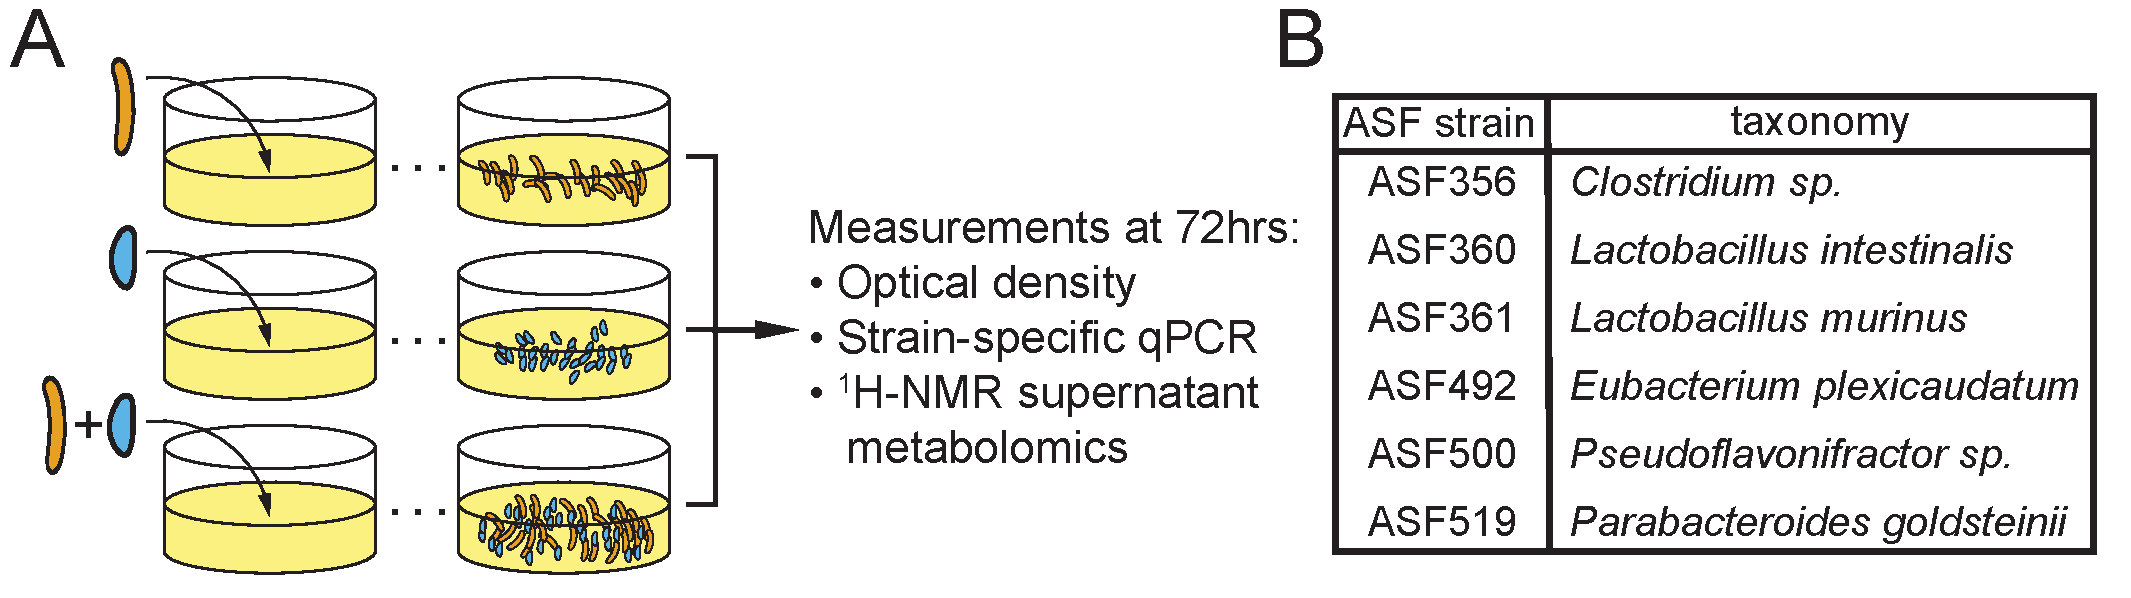
\includegraphics[width=\textwidth]{ch2_fig1}
\caption[Summary of co-culture experiment design, measurements, and total growth outcomes in monocultures and co-cultures.]{\textbf{Summary of co-culture experiment design, measurements, and total growth outcomes in monocultures and co-cultures.} \textbf{A)} Experimental procedure for each pair of strains and measurements taken. \textbf{B)} Taxonomic assignment for strains included in this study.}
\end{figure*}

The altered Schaedler flora (ASF) is a group of 8 bacterial strains isolated from the mouse gastrointestinal tract used to standardize the microbiota of laboratory mice \cite{Wymore_Brand2015-ez}. ASF-colonized mice remain stably colonized across mouse generations and have normalized organ physiology relative to germ-free mice \cite{Wymore_Brand2015-ez}. Although there are known differences between the immune repertoires of ASF-colonized mice and conventional mice, these differences can be exploited to test specific hypotheses \cite{Geuking2011-fj,Ivanov2009-vl}. ASF mice have been used widely in infectious disease research to study Clostridium difficile \cite{Schwan2009-zo}, Salmonella enterica \cite{Brugiroux2016-vi}, and Cryptosporidium parvum \cite{Harp1992-wr}. Many specific pathogen-free mice are initially colonized with the ASF, which has led to the theory that presence or absence of ASF strains contributes to vendor-specific differences in susceptibility to disease \cite{Singer2000-tr}.  Further use of gnotobiotic systems such as ASF-colonized mice could greatly accelerate discovery in microbiome research, especially if the behavior of the ASF alone is well-understood.

Previously, we performed pairwise spent media experiments using seven of the ASF strains, in which each strain was grown in the same medium as well as the spent medium of other strains \cite{Biggs2017-fs}. We identified cases of putative cross-feeding and competition and the effect of those interactions on growth dynamics. However, each strain was spatially and temporally separated in that study. While spent media experiments remove some technical and statistical complications in inferring metabolic interactions, the interactions that are possible are different than those that might occur while strains are grown in co-culture.

Here, we further define the interactive potential of six of the ASF strains and develop an analytic method to infer putative mechanisms of metabolic interaction. We perform co-culture growth experiments with all pairs of these strains and profile their supernatant metabolomes in both mono- and co-culture. We identify the influence of interspecies interactions on growth of each strain, then apply our analytic framework for inferring putative metabolic mechanisms of interaction from supernatant metabolomic data. We experimentally interrogate an inferred cross-feeding interaction in which one ASF strain (Parabacteroides goldsteineii ASF519) produces amino acids that another (Clostridium sp. ASF356) consumes, confirming that the hypothesized mechanism occurs and leads to a growth benefit for the consuming strain. With this new insight, we provide a framework to identify putative metabolic mechanisms of microbe-microbe and host-microbe interactions that can be applied to any microbial community to investigate co-culture phenotypes including growth enhancement or changes in metabolite yield.

\section{Results}
\subsubsection{Ecological interactions within the altered Schaedler flora}

We collected \textit{in vitro} data for growth of all pairwise combinations of 6 ASF strains (\textbf{Figure 2.1A}, n=6-9 per strain pairing). Taxonomic assignments for these strains are provided in \textbf{Figure 2.1B}. We determined the impact of co-culture on each strains’ growth by comparing monoculture abundance after 72 hours of growth to the abundance of each strain in co-culture at the same time (determined using probe-based qPCR; all strains are in stationary phase; see example growth curves in \textbf{Supplemental Figure 2.2}; see Methods).

\begin{figure*}
\centering
\includegraphics[width=0.95\textwidth]{ch2_fig2}
\caption[The effects of pairwise co-culture on the abundance of each strain.]{\textbf{The effects of pairwise co-culture on the abundance of each strain.} \textbf{A)} Relative abundance of each strain in monoculture and co-culture determined via qPCR. Abundance is plotted on linear scale, not log-transformed. x-axis describes abundance of strain at the bottom of the column; y-axis describes abundance of strain left of each row. Diamonds indicate abundance of each strain in monoculture, with mean shown by a dashed line. Abundance of each strain in co-culture as indicated by the row and column labels is shown by a black circle, with mean abundances indicated by grey dashed lines. Abundance for each strain is z-score normalized using mean and standard deviation of monoculture abundance to center and scale the data, respectively. N=9 for all samples except for those with Pseudoflavonifractor ASF500 or Eubacterium ASF492, for which N=6. \textbf{B)} Heatmap of mean abundance of each strain in co-culture relative to monoculture. Blue indicates less abundant, while red indicates more abundant, than monoculture. The upper left and lower right triangles in each square describes abundance of the strain labelled on the left of row and bottom of column, respectively. White circles indicate differential abundance between monoculture and co-culture (\textit{p} \textless\! 0.10, Mann-Whitney U test with false discovery rate correction using Benjamini-Hochberg procedure). \textbf{C)} Summary of interspecies interactions. Non-zero interactions in the triangular matrix indicate significant differential abundance as shown in \textbf{Figure 2.2B}.}
\end{figure*}

Abundance of each strain in each pair was evaluated to determine whether a negative (-), positive (+), or neutral (0) effect on abundance occurred in the pairing, allowing classification of pairwise interaction with standard ecological terminology. All pairings except one, \textit{Clostridium} ASF356 with \textit{Parabacteroides} ASF519, had a negative impact on the abundance of at least one strain, with 0/- (amensalism), +/- (parasitism), -/- (competition), and +/0 (commensalism) being the only interactions detected (8, 4, 2, and 1 instances, respectively; data shown in \textbf{Figure 2.2A}, summarized in \textbf{Figure 2.2B} and \textbf{2.2C}). \textit{Lactobacillus} ASF361 was present in 3/4 parasitic co-cultures and experienced a growth benefit in all cases. In contrast, growth of both \textit{Eubacterium} ASF492 and \textit{Pseudoflavonifractor} ASF500 was inhibited in every condition, including in co-culture with each other. In summary, abundance of individual strains tended to be lower in co-culture than in monoculture. However, the growth benefit observed for some strains also suggests that differences in resource utilization across strains, or emergent behavior in co-culture such as cross-feeding and consumption of novel substrates/metabolites, occurred in some co-cultures.

\subsubsection{Metabolic repertoires within the altered Schaedler flora}

\begin{figure*}[t]
\centering
\includegraphics[width=\textwidth]{ch2_fig3}
\caption[Metabolic behavior of each strain in monoculture and emergent behavior in co-cultures.]{\textbf{Metabolic behavior of each strain in monoculture and emergent behavior in co-cultures.} \textbf{A)} Heatmap describing supernatant metabolomes for each monoculture. Red/blue indicate higher/lower concentrations than fresh medium, respectively. Values are centered at 0 using the mean in fresh media, then scaled between -1 and +1 by dividing by the maximum change in concentration for each metabolite in any sample in the study. Unnamed metabolites not shown. Hierarchical clustering was performed using Euclidean distances and complete linkage. \textbf{B-E)} Principal component analysis (PCA) of monocultures and co-culture, performed independently for each subplot. Sky blue/orange circles correspond to monoculture supernatant metabolomes from strain labelled with same color. Co-culture samples for the two strains in each subplot title are indicated by grey circles. Percent variance captured by each principal component is labelled on each axis.}
\end{figure*}

To determine potential mechanisms governing the changes in growth observed in co-culture, we performed metabolomics on the spent supernatant from all samples in the growth experiments (using  $^1\!$H NMR spectroscopy, see Methods). We updated and refined the metabolite peak annotations from experiments previously performed using the same medium and strains \cite{Biggs2017-fs}, resulting in 86 detected metabolites, 50 of which could be assigned an identity (36 of 85 metabolites were previously assigned an identity). We identified new metabolites involved in amino acid metabolism (serine, cystine, asparagine, glutamate, 2-oxoisocaproate, and isocaproate), nucleic acid metabolism (cytidine, cytosine, uridine monophosphate), and anaerobe-specific metabolism (isopropanol).

Based on the monoculture supernatant metabolomic profiles presented here (\textbf{Figure 2.3A}) and in our previous study of the ASF, the ASF strains have fermentation repertoires similar to closely-related gut microbes \cite{Biggs2017-fs}. \textit{Lactobacillus} ASF360 and \textit{Lactobacillus} ASF361 both produced lactate, while \textit{Lactobacillus} ASF361 also produced acetate and formate. Other strains of \textit{Lactobacillus intestinalis} and \textit{Lactobacillus murinus} are generally identified as facultative heterofermentative lactic acid bacteria \cite{Vos2011-bf}. Heterofermentative lactic acid bacteria ferment carbohydrates to lactate but may also produce additional acetate in some conditions. \textit{Clostridium} ASF356 produced the common fermentation end products acetate, propionate, succinate, and butyrate. Butyrate production is common in \textit{Clostridia} that inhabit mammalian gastrointestinal tracts, and is often coupled with acetate production \cite{Louis2009-ax}. Propionate is the primary end product of three common pathways identified in anaerobic organisms, of which the acrylate pathway and succinate pathway have been identified in \textit{Clostridia spp.} \cite{Reichardt2014-ua}. \textit{Clostridium} ASF356 also produced isovalerate, isocaproate, and isobutyrate, which are common products of amino acid fermentation by some \textit{Clostridia spp.} \cite{Mead1971-oa}.

Butyrate and ethanol were the only common fermentation end products produced by \textit{Eubacterium} ASF492. \textit{Eubacterium} ASF492 has been proposed as the type strain for \textit{Eubacterium plexicaudatum} \cite{Dewhirst1999-pp}, which was originally identified as producing butyrate and small amounts of acetate from glucose \cite{Wilkins1974-yn}. \textit{Pseudoflavonifractor} ASF500 produced only formate and consumed less lactose than any other ASF strain, suggesting that lactose is not a preferred carbon source for \textit{Pseudoflavonifractor} ASF500 or another growth-limiting nutrient is only present at low abundance in the medium. \textit{Parabacteroides} ASF519 produced acetate, propionate, and succinate, consistent with previous reports on fermentation products of \textit{Parabacteroides goldsteinii} \cite{Song2005-mt}, as well as formate. \textit{Parabacteroides} ASF519 also produced many amino acids, including histidine, lysine, alanine, isoleucine, valine, proline, phenylalanine, glutamate, and methionine, suggesting \textit{Parabacteroides} ASF519 contains a comprehensive amino acid biosynthesis repertoire.

\subsubsection{Co-culture can lead to emergent metabolic behavior}

Co-culture substantially altered the metabolome of pairings relative to each of the monoculture metabolomes for the strains involved (see \textbf{Supplemental Figure 2.1} for results from all groups). To detect and quantify the emergent metabolic behavior resulting from co-culture, we performed principal component analysis (PCA; see Methods) on the metabolic profile for pairs of strains. We performed PCA separately for each pair of strains, including samples from each monoculture and the co-culture. In cases where both strains grew in co-culture (i.e. no strong negative growth effect), the first principal component (PC1) separated monocultures by strain and the second principal component (PC2) separated monoculture samples from co-culture samples. This behavior was particularly strong in the case of \textit{Clostridium} ASF356 and \textit{Parabacteroides} ASF519 (\textbf{Figure 2.3B}). For \textit{Clostridium ASF356} and \textit{Parabacteroides} ASF519, the loadings of PC2 suggest that co-culture increased production of propionate, glycine, and the amino acid fermentation products isovalerate, isocaproate, and isobutyrate, and increased consumption of multiple amino acids and lactose.

For pairings with a strong negative effect on one strain, the co-culture metabolomes were less similar to the negatively-affected strain than the other strain. For example, co-culture of \textit{Clostridium ASF356} with \textit{Lactobacillus} ASF360 resulted in decreased growth of \textit{Lactobacillus} ASF360, and the co-culture samples are located closer to \textit{Clostridium} ASF356 monoculture samples in PCA (\textbf{Figure 2.3C}). Although there is still an “emergent” co-culture effect observed in PC2 for this pair, the effect is also aligned with within-group variation. The same trend is present for \textit{Lactobacillus} ASF361, \textit{Parabacteroides} ASF519, and their co-culture (\textbf{Figure 2.3D}). For strong negative growth outcomes (e.g. \textit{Clostridium} ASF356 and \textit{Lactobacillus} ASF361 co-culture), the effect is more pronounced and there is less separation between monoculture and co-culture samples (\textbf{Figure 2.3E}).

\subsubsection{Development of an expectation-based model to account for changes in strain abundance}

Based on the metabolic differences between monoculture and co-culture samples identified via PCA, co-culture conditions substantially altered metabolic behavior. However, the mechanism that leads to this emergent metabolic behavior is unclear, and attempting to infer the mechanism may be confounded by changes in the abundance of each strain in co-culture. We sought to infer metabolic interactions between strains in co-culture by accounting for changes in strain abundance. While the absolute amount of a metabolite produced or consumed may change in co-culture relative to monoculture, taking changes in strain abundance into account is necessary to determine whether the change in metabolite abundance is emergent behavior rather than additive.

\begin{figure*}[tb!]
\centering
\includegraphics[width=0.95\textwidth]{ch2_fig4}
\caption[Accounting for co-culture growth outcomes with ConYE to identify emergent metabolism.]{\textbf{Accounting for co-culture growth outcomes with ConYE to identify emergent metabolism.} \textbf{A)} Procedure for the constant yield expectation (ConYE) model. \textbf{B)} Examples of ConYE results for Lactose, Lactate, Valine, and Proline. Diagonal shows monoculture behavior for each strain. Every pair of triangles indicates the observed metabolite abundance in co-culture (lower left), the expected metabolite abundance (upper right), and whether there was a significant difference between observed and expected values. Centering and scaling performed as in \textbf{Figure 2.3}, except expected values were included while selecting a max value. Mann-Whitney U-Test with false discovery rate (FDR) control using the Benjamini-Hochberg procedure was performed for all 1290 comparisons (15 co-cultures, 86 metabolites each). Asterisk indicates p \textless\! 0.05 for the metabolite in the co-culture containing the indicated strains. \textbf{C)} ConYE results for all strain pairings for metabolites that were consumed by one or both strains in monoculture (left, blue), produced by one or both strains in monoculture (middle, red), or produced by one strain in monoculture and consumed by the other strain in monoculture (right, green). Each point represents a metabolite in a co-culture pair. x axis show the difference between observed and expected metabolite abundance in co-culture (scaled as in panel B), and y axis shows the p-value from ConYE. Points above grey line have p \textless\! 0.05. Percentage of points in the labelled quadrant relative to the rest of the points in the subplot is shown.}
\end{figure*}

We developed a Constant Yield Expectation (ConYE) model to identify metabolites for which consumption or production behavior changed in co-culture (see Methods). Within the ConYE model, we assume each strain produces or consumes a fixed quantity of each metabolite per unit biomass (i.e. constant yield), then test whether that assumption is true in co-culture by comparing the expected behavior to the observed co-culture data. We simulate expected metabolite quantities in co-culture by multiplying the mono-culture-derived metabolite yield for each strain by the observed abundance of that strain in co-culture, then summing the expected values for each strain and the initial quantity of the metabolite present in the fresh medium (\textbf{Figure 2.4A}). For each metabolite, we test the null hypothesis that the quantity of that metabolite in co-culture is equal to that predicted by the ConYE model. Rejecting the null hypothesis for a metabolite implies that co-culture caused at least one strain to alter metabolism of that metabolite relative to its own biomass production.

We identified several patterns with the ConYE model results that were consistent across sets of many metabolites, for which representative examples are shown (\textbf{Figure 2.4B}). Metabolites consumed in monoculture were often consumed less than expected in co-culture, especially when one strain in the co-culture experienced a growth benefit (e.g. lactose). For some strains, this pattern may arise because alternative metabolites are now available in co-culture that can be consumed to produce biomass, decreasing the amount of lactose required to produce a unit of biomass. Similarly, another pattern involves fermentation end products, which were generally less abundant than expected. Lactate, which was produced by \textit{Lactobacillus} ASF360 and \textit{Lactobacillus} ASF361, was less abundant than expected in 7/9 co-cultures containing either strain. Explanations for this pattern align with explanations for the first pattern; individual strains may utilize alternative metabolites to produce biomass, resulting in less production of primary fermentation products. An alternative explanation is that other strains in the co-culture are consuming the fermentation end product, as may be the case for lactate (\textit{Clostridium} ASF356, \textit{Eubacterium} ASF492, and \textit{Parabacteroides} ASF519 consumed lactate in the fresh medium). Similar explanations may fit the behavior of other metabolites that are not end products of fermentation, such as valine. Valine was consumed by some strains and produced by others, but the null hypothesis for valine was only rejected for 3/15 co-cultures. In cases where one strain produced a metabolite in monoculture (e.g. \textit{Parabacteroides} ASF519 producing valine) and another strain consumed the metabolite in monoculture (e.g. \textit{Clostridium} ASF356 consuming valine), failure to reject the null hypothesis even when one strain experienced a growth benefit (e.g. \textit{Clostridium} ASF356 co-cultured with \textit{Parabacteroides} ASF519) suggests that a metabolite may have been cross-fed.

As demonstrated by these examples, interpretation of ConYE can be informed by considering the direction of metabolite abundance change in monoculture. If either strain consumed a metabolite in monoculture (\textbf{Figure 2.4C}, left, all co-cultures shown), rejecting the null hypothesis implies the metabolite was consumed more or less than expected, or that one of the strains produced the metabolite in co-culture (e.g. emergent production). Conversely, if either strain produced a metabolite in monoculture (\textbf{Figure 2.4C}, middle), rejecting the null hypothesis implies the metabolite was produced more or less than expected, or that one of the strains consumed the metabolite in co-culture (which was not observed in monoculture for that strain). For both the production and consumption cases, cross-feeding is still possible, but requires emergent consumption or production by one strain.

When a metabolite was consumed by one strain in monoculture and produced by the other strain in monoculture (\textbf{Figure 2.4C}, right), there are four possible interpretations if the null hypothesis is rejected. If the metabolite was less abundant than expected, then at least one of two conclusions is true: 1) the consumer metabolized more of the metabolite than expected, or 2) the producer produced less. If the metabolite was more abundant than expected, the opposite is true (producer produced more or consumer consumed less). If the null hypothesis is not rejected, the strains either maintained their production and consumption behavior from monoculture, or both scaled their consumption and production up or down in equal amounts. These interpretations, as well as their corresponding importance or relative contribution to a positive growth interaction for the consuming strain, are summarized in \textbf{Figure 2.5}.

\begin{figure}[tb]
\centering
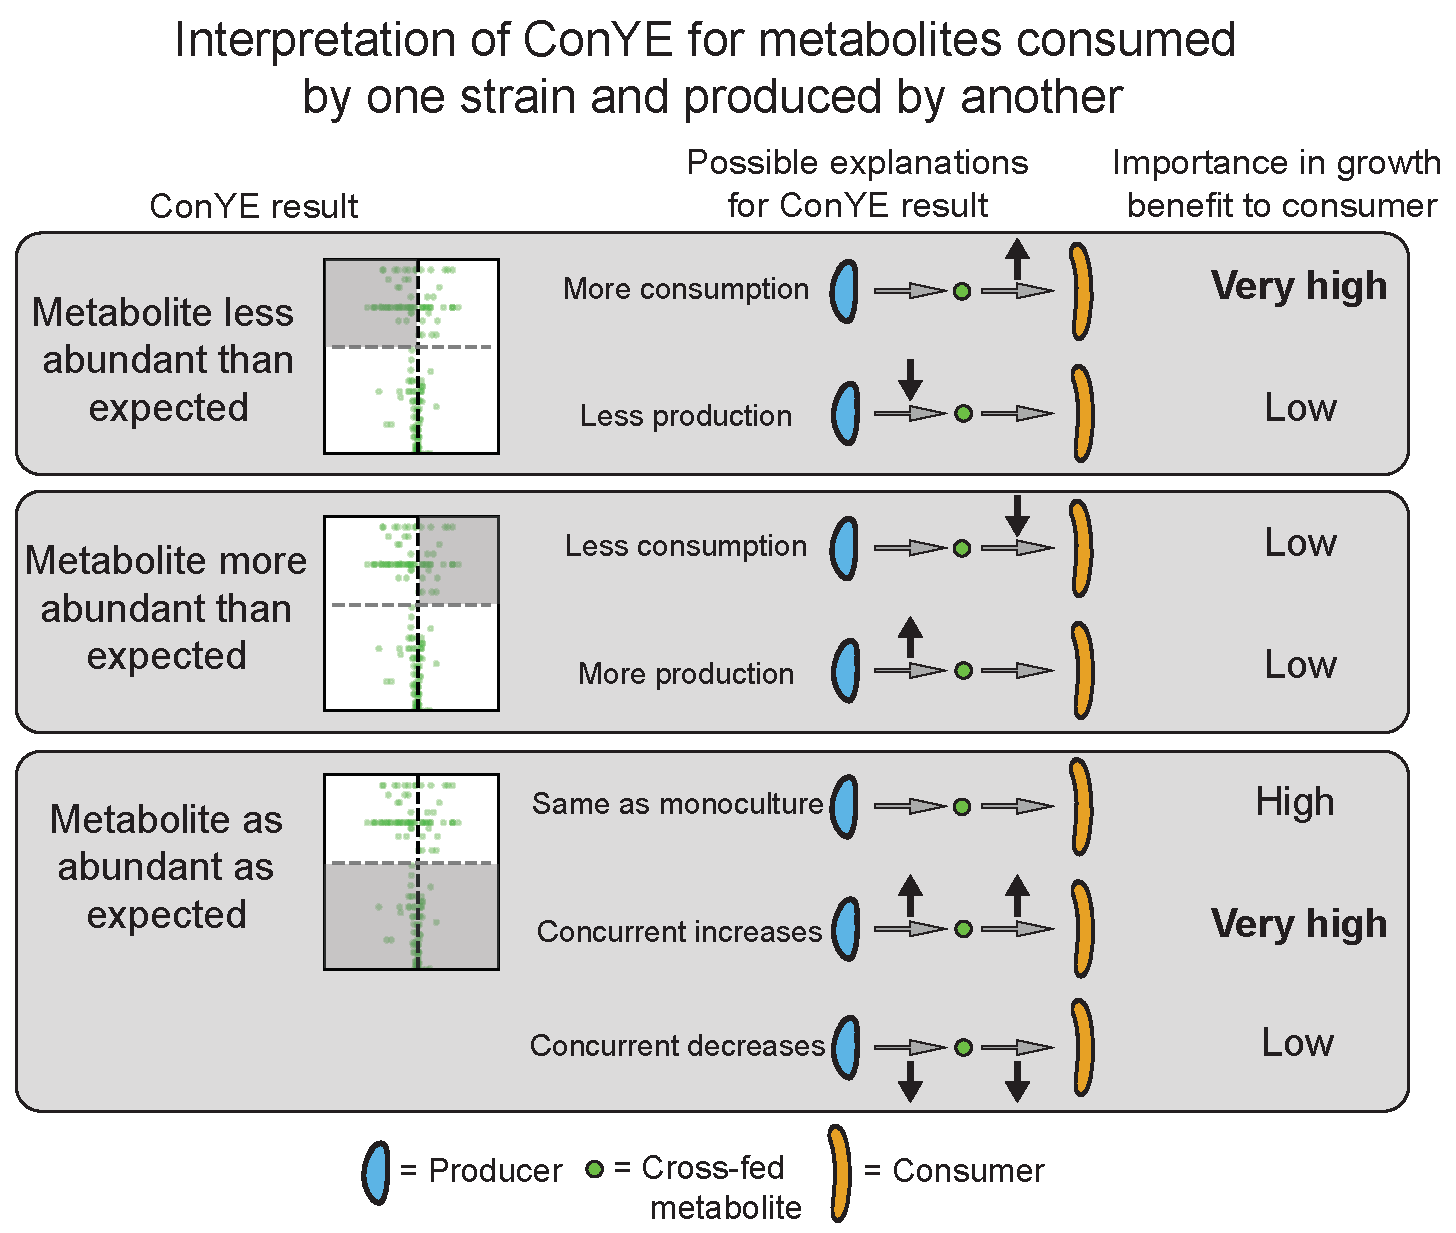
\includegraphics[width=\linewidth]{ch2_fig5}
\caption[Interpretations of ConYE results for metabolites consumed by one strain in monoculture and produced by another strain in monoculture.]{\textbf{Interpretations of ConYE results for metabolites consumed by one strain in monoculture and produced by another strain in monoculture.} In this example, the consumer experienced a growth benefit. The shaded region of each volcano plot describes the points that fall into the category described on left. In “Importance in growth benefit to consumer” column, the entry for each scenario assumes that consumption of the metabolite is coupled with biomass production. The importance assignments are qualitative, and reflect whether the consumer experienced an increase in metabolite flux in the explanatory scenario (high for increased flux, low for decreased flux).}
\end{figure}

\subsubsection{Co-culture increases the efficiency of metabolite utilization}

After applying ConYE to all co-cultures, the null hypothesis was rejected for 500/1290 metabolites (38.8\%; 86 metabolites tested across 15 co-culture conditions, resulting in 1290 comparisons), suggesting that co-culture alters metabolism of a substantial portion of metabolites when taking into account changes in growth during co-culture. For metabolites that were consumed by one or both strains in monoculture, the amount consumed per unit of strain growth generally decreased in co-culture if the null hypothesis was rejected. Specifically, of the 624 instances of metabolites that fell into this category, 151 (24.2\%) were significantly more abundant than expected in co-culture, whereas 94 (15.1\%) were less abundant than expected (\textbf{Figure 2.4C}, left). Of the 278 instances of a metabolite being produced by one or both strains in a pairing in monoculture, 71 (25.5\%) were less abundant than expected, while 27 (9.7\%) were more abundant than expected (\textbf{Figure 2.4C}, middle). Thus, although co-culture often resulted in a greater quantity of a metabolite being produced relative to either monoculture (i.e. metabolites driving monoculture and co-culture separation in PCA, \textbf{Figure 2.3B}), the amount produced relative to growth of each strain decreased for most metabolites. Similarly, the amount of each metabolite consumed relative to biomass in co-culture generally decreased. These results suggest that these co-cultures can increase the efficiency of biomass production through niche expansion (e.g. consuming metabolites they did not consume in monoculture) or cross-feeding rather than increasing consumption of metabolites they did not fully deplete in monoculture. Indeed, 90/1290 (6.98\%) metabolites were not consumed or produced by either strain in monoculture, yet were consumed when the two strains were in co-culture.

These distinct ConYE trends are enriched in cases with positive growth interactions (\textbf{Figure 2.6A}). When considering only pairings with a positive growth effect for at least one strain, there were 219 metabolites that were consumed by one or both strains in monoculture. Of these 219 metabolites, 138 (63.0\%) were more abundant than expected, while only 6 (2.74\%) were less abundant than expected. Of the 88 metabolites produced by one or both strains in monoculture for these co-cultures, 51 (58.0\%) were less abundant than expected, and only 5 (5.68\%) were more abundant than expected. Taken together, these results indicate that co-cultures with positive interactions are able to more efficiently utilize resources than co-cultures without positive interactions or monocultures.

There are three mechanisms that may enable this phenotype: niche expansion (consumption of metabolites not consumed in monoculture), cross-feeding, and detoxification via consumption of growth-inhibiting metabolites. In co-culture, the subset of strain pairs with positive interactions consumed 30 metabolites that were not consumed by either species in monoculture. Interestingly, all 30 instances of emergent metabolite consumption were carried out by \textit{Lactobacillus} ASF361+\textit{Eubacterium} ASF492, \textit{Lactobacillus} ASF361+\textit{Pseudoflavonifractor} ASF500, and \textit{Eubacterium} ASF492+\textit{Parabacteroides} ASF519, while the remaining two pairs (\textit{Clostridium} ASF356+\textit{Parabacteroides} ASF519 and \textit{Lactobacillus} ASF361+\textit{Parabacteroides} ASF519) had 0 cases of emergent consumption (See Table S3 for all cases). Given this result, it is likely that the growth benefits that occurred for \textit{Clostridium} ASF356+\textit{Parabacteroides} ASF519 and \textit{Lactobacillus} ASF361+\textit{Parabacteroides} ASF519 are due to cross-feeding or detoxification, while the growth benefits for the other positive interaction pairs are at least in part due to niche expansion.

\begin{figure*}[tb!]
\centering
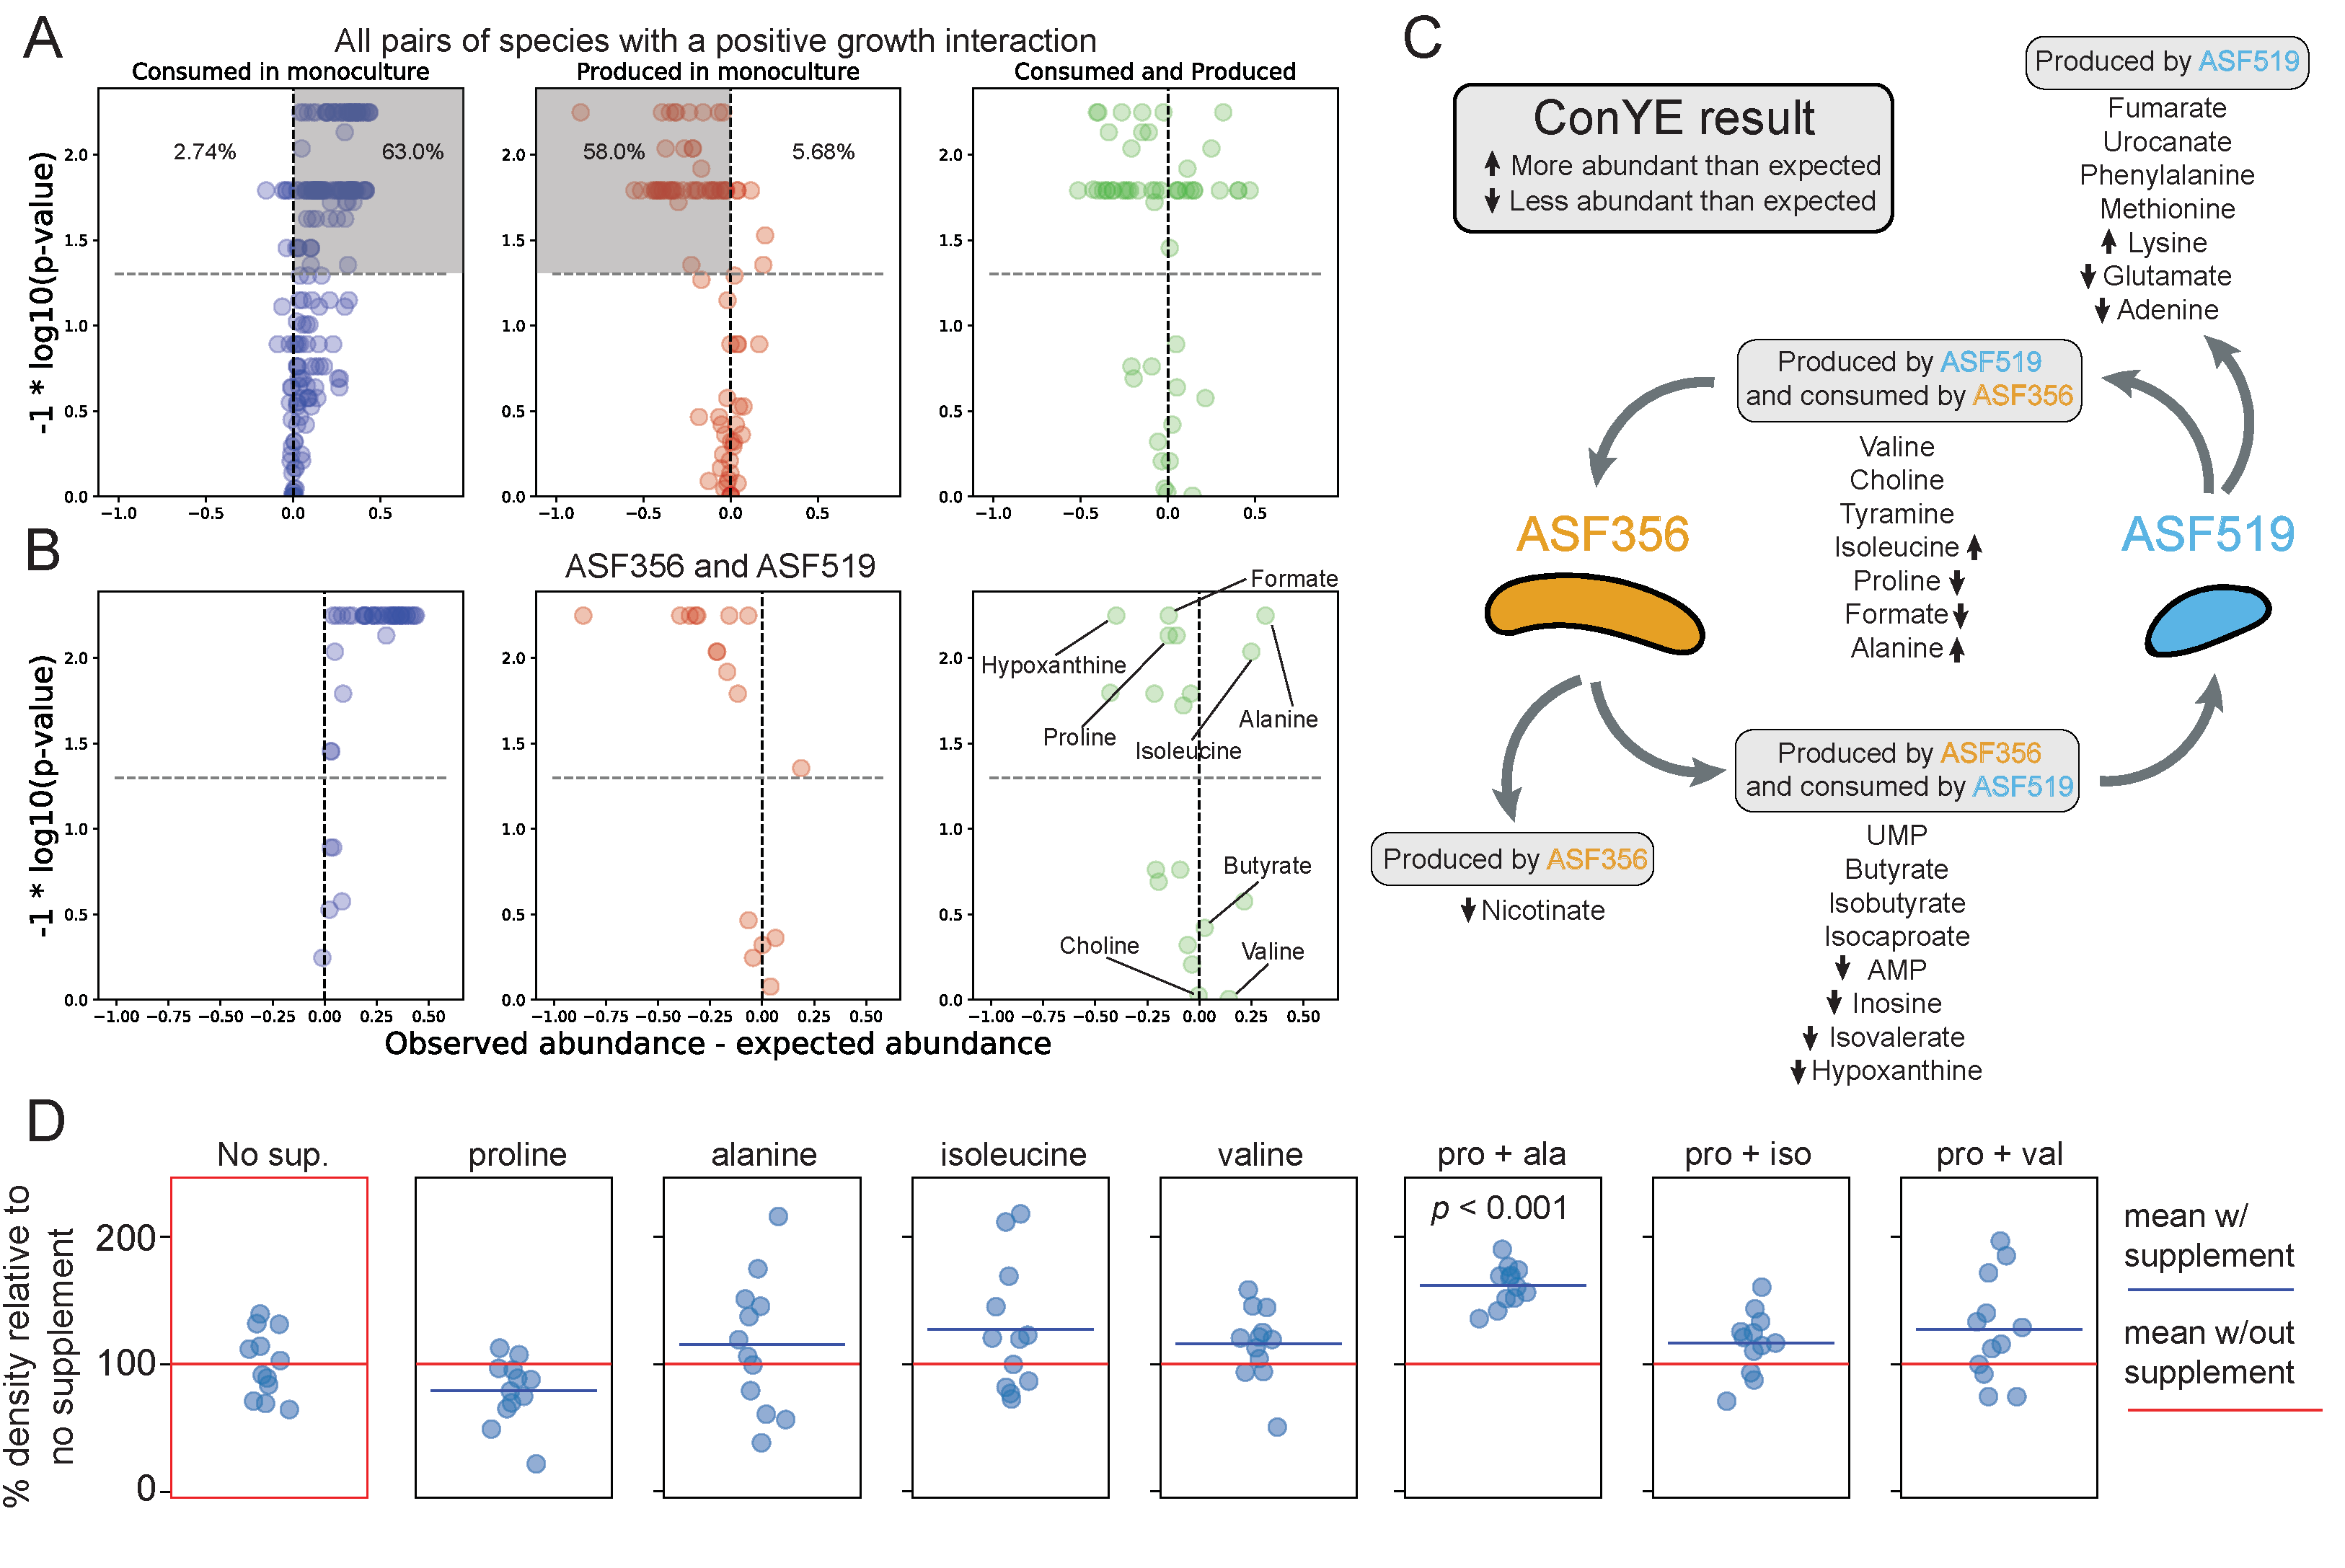
\includegraphics[width=\textwidth]{ch2_fig6}
\caption[Emergent metabolism in co-culture pairings with a growth benefit and in vitro testing.]{\textbf{Emergent metabolism in co-culture pairings with a growth benefit and in vitro testing.} \textbf{A)} ConYE results for all metabolites from co-cultures with a positive growth interaction. Shaded quadrants represent consumed metabolites that were more abundant than expected (left) or less abundant than expected (middle). Percentages shown represent the number of metabolites within the plot that fall in the quadrant. \textbf{B)} ConYE results for co-culture of Clostridium ASF356 and Parabacteroides ASF519. Metabolites on right for which p \textgreater\! 0.05 are labeled unless they could not be assigned an identity. Metabolites for which p \textless\! 0.05 are labeled if assigned an identity and abs(x) \textgreater\! 0.10 for that metabolite. x and y axes are scaled as in \textbf{Figure 2.4}. \textbf{C)} Metabolic interaction topology for Clostridium ASF356 and Parabacteroides ASF519. ConYE results are indicated with arrows pointing up or down for metabolites for which the null hypothesis was rejected. Metabolite classifications are based on monoculture behavior. \textbf{D)} OD600 of Clostridium ASF356 monocultures after 72 hours of growth in supplemented media conditions. ”No sup.” had no supplement added, while conditions with a single amino acid were supplemented at 1.25g/L. In conditions with two supplements, each metabolite is supplemented at 1.25g/L. “pro + ala”, “pro + iso”, and “pro + val” conditions include L-proline with L-alanine, L-isoleucine, or L-valine, respectively.}
\end{figure*}

\subsubsection{Identifying cross-fed metabolites and evaluating feasibility \textit{in silico}}

We next sought to investigate potential cross-fed metabolites from ConYE for co-cultures with positive growth interactions in order to find a mechanism that explained, at least in part, the growth benefit. For this task, we focused on the co-culture of \textit{Clostridium} ASF356 and \textit{Parabacteroides} ASF519 to exclude co-cultures which may have engaged in niche expansion (and therefore cross-feeding may have played a more minor role in observed growth benefits) and to remove the need to consider additional confounding factors introduced by a strong negative growth interaction (e.g. negative impact on \textit{Parabacteroides} ASF519 growth in co-culture with \textit{Lactobacillus ASF361}). Seven named metabolites were consumed by \textit{Clostridium} ASF356 in monoculture that were also produced by \textit{Parabacteroides} ASF519 in monoculture (\textbf{Figure 2.6B}; labelled metabolites satisfy criteria specified in figure caption). Of those 7 metabolites, tyramine, valine, and choline did not result in rejecting the ConYE null hypothesis. Isoleucine and alanine were more abundant than expected, and proline and formate were less abundant than expected. Isoleucine and alanine may have been cross-fed, but given that they were more abundant than expected, consumption of these metabolites only contributed to enhanced growth if \textit{Parabacteroides} ASF519 also produced less of these metabolites than expected (as in middle panel of \textbf{Figure 2.5}, where \textit{Parabacteroides} ASF519 is the producer and \textit{Clostridium} ASF356 is the consumer). Proline and formate were both less abundant than expected, so were either consumed by \textit{Clostridium} ASF356 more in co-culture than in monoculture (and thereby cross-fed) or produced less by \textit{Parabacteroides} ASF519 in co-culture than in monoculture (as in top panel of \textbf{Figure 2.5}).

ConYE can identify metabolites that are potentially cross-fed, but the actual behavior of each strain in co-culture with respect to that metabolite is difficult to infer using existing experimental techniques. Because we can only evaluate the co-culture behavior based on an expectation derived from monoculture behavior, it is still possible that co-culture leads to reduced production and consumption of those metabolites rather than cross-feeding. We sought to provide orthogonal evidence for ConYE results by evaluating the potential for metabolites to increase the growth rate of a strain in monoculture, reasoning that ConYE may produce false-positive inferences if metabolites are not actually coupled with biomass production. We chose to support inferences made using ConYE by building and applying Genome-scale metabolic network reconstructions (GENREs). GENREs are mathematical representations of all metabolic reactions that an organism can carry out, and have been used extensively to predict the effect of environmental conditions on growth of bacterial species \cite{Oberhardt2009-iu}. We created an ensemble of 100 GENREs for each strain in this study to gain greater confidence in cross-feeding predictions and to enable predictive modeling of metabolism in future studies (\textbf{Figure 2.7A-B}; see Methods). For each metabolite, we evaluated its impact on growth of individual strains by performing ensemble flux balance analysis (EnsembleFBA \cite{Biggs2017-md} to predict the growth rate of the strain without the metabolite available and with the metabolite available in excess (see Methods). We performed this procedure for the cross-feeding candidate metabolites between \textit{Clostridium} ASF356 and \textit{Parabacteroides} ASF519. If a metabolite increases the predicted \textit{in silico} growth rate when available in excess, we take that as parallel evidence to support or oppose the ConYE-based inferences. EnsembleFBA results are summarized in \textbf{Figure 2.7C} for all metabolites except tyramine, which was not present in any GENREs within the ensemble for \textit{Clostridium} ASF356.

\begin{figure*}[tb]
\centering
\includegraphics[width=0.8\textwidth]{ch2_figS3}
\caption[Computational model-driven interrogation of potential metabolic interactions and experimental validation of a cross-feeding interaction.]{\textbf{Computational model-driven interrogation of potential metabolic interactions}  \textbf{A)} Process for generating and applying a genome-scale metabolic network reconstruction (GENRE). \textbf{B)} Novel pipeline for constructing and analyzing ensembles of GENREs for the ASF strains. Details for each step in Methods. \textbf{C)} EnsembleFBA predictions of the influence of potentially cross-fed metabolites on growth of \textit{Clostridium} ASF356. Biomass production values are for flux through the biomass reaction in units of hour-1, and a metabolite was considered essential if removal led to flux through the biomass reaction of less than \textless\! 1E-5/hour. Predicted flux through biomass in the experimental medium without any supplement or metabolite removal is 0.079/hour.}
\end{figure*}

Valine was essential for growth of \textit{Clostridium ASF356} in all 100 GENREs in its ensemble. Isoleucine was essential for 85/100 GENREs but had no effect on growth for the other 15 GENREs, while absence of the rest of the potentially cross-fed metabolites had no effect on predicted growth rate. Given the \textit{in silico} essentiality of valine and the ConYE results indicating valine was as abundant as expected, valine may have conferred a growth benefit to \textit{Clostridium} ASF356 if cross-fed between \textit{Clostridium} ASF356 and \textit{Parabacteroides} ASF519. While isoleucine was essential for growth of the majority of GENREs in the \textit{Clostridium} ASF356 ensemble, there was a subset of GENREs in which its removal had no effect. Given this \textit{in silico} uncertainty, as well as the ConYE result which indicated it was more abundant than expected in co-culture, we hypothesized that cross-feeding of isoleucine may not have influenced growth of \textit{Clostridium} ASF356 as much as valine. Alanine, proline, choline, and formate were not essential and did not influence predicted growth rates \textit{in silico}. Critically, however, this analysis indicated that availability of any of the individual metabolites in excess did not confer a growth benefit relative to the unsupplemented medium.

\subsubsection{\textit{In vitro} investigation of an inferred cross-feeding interaction}

Given the lack of an \textit{in silico} prediction which indicated that supplementation of a putatively-crossfed metabolite would increase the growth rate of \textit{Clostridium} ASF356, we considered mechanisms through which the metabolites discussed above may interact with each other to influence growth, rather than in isolation as considered thus far. \textit{Clostridium} ASF356 belongs to the \textit{Clostridium} genus, throughout which amino acid fermentation via Stickland reactions is common \cite{Mead1971-oa}. Stickland reactions involve coupling the oxidative deamination of one amino acid with the reductive decarboxylation of another amino acid, producing two short-chain fatty acids or branched chain fatty acids that each contain one fewer carbon than the respective amino acid from which they were derived \cite{Nisman1954-xl}. Proline, glycine, hydroxyproline, and ornithine are strong Stickland reaction electron acceptors, while alanine, valine, leucine, and isoleucine are strong electron donors. We observed that \textit{Clostridium} ASF356 consumed proline, a strong electron acceptor, and all the listed electron donors in monoculture, while \textit{Parabacteroides} ASF519 produced proline, alanine, valine, and isoleucine and consumed leucine in monoculture. In co-culture, ConYE indicated that proline was significantly less abundant than expected, suggesting it was consumed more per unit biomass in co-culture than in monoculture. Given this observation and the lack of growth rate increase predicted \textit{in silico} with excess proline available, we hypothesized that proline was of critical importance to the growth benefit for \textit{Clostridium ASF356} in co-culture with \textit{Parabacteroides} ASF519, but depended on the presence of suitable electron donors. Behavior varied amongst the electron donors that may pair with proline in the Stickland reaction: isoleucine and alanine were more abundant than expected, while valine was as abundant as expected. The Stickland fermentation product for proline is 5-aminovalerate, which we could not identify within the NMR spectra due to spectral overlap with other metabolites and lack of signal in regions unique to 5-aminovalerate. The products for isoleucine, valine, and alanine are valeric acid (not detected), isobutyrate (as abundant as expected), and acetate (less abundant than expected), respectively. Decreased abundance of leucine, which is fermented to isovalerate (less abundant than expected), in co-culture suggests decreased consumption by \textit{Clostridium} ASF356 or increased consumption of isovalerate by \textit{Parabacteroides} ASF519, which consumed isovalerate in monoculture.

To test the hypothesis that \textit{Clostridium} ASF356 experiences a growth benefit in the presence of proline and suitable electron donors, we grew \textit{Clostridium} ASF356 in media supplemented with proline, alanine, isoleucine, valine, or each combination of the three electron donors (alanine, isoleucine, valine) with proline. NMR spectroscopy cannot differentiate between amino acid isomers, so we assumed all amino acids consumed and produced were the L- isoform (as in tryptone, the major source of amino acids in the medium). Organisms conducting Stickland fermentation of proline generally possess a proline racemase, since D-proline is the isoform that is fermented \cite{Watanabe2015-wa}. Leucine was consumed by both strains in monoculture, thus was excluded because it was unlikely to be cross-fed in co-culture. Only the monoculture supplemented with both proline and alanine had increased density relative to no supplement (\textbf{Figure 2.6D}, \textit{p} \textless\! 0.05, Mann-Whitney U-test with false discovery rate control using Benjamini-Hochberg procedure), suggesting that co-metabolism of proline and alanine contributes to growth of \textit{Clostridium} ASF356. Given that the ConYE results indicated that alanine was more abundant in co-culture than expected, the results of the supplementation experiment imply that production of alanine by \textit{Parabacteroides} ASF519 was increased in co-culture with \textit{Clostridium} ASF356 or that \textit{Clostridium} ASF356 used alanine more efficiently in co-culture. Additionally, the lack of growth benefit conferred by supplementation of proline with isoleucine or valine suggests that any change attributable to pairing either electron donor with proline was too small to detect given our sample size. Formate can also be used as an electron donor for proline reduction in the Stickland reaction \cite{Kabisch1999-jf}, which we did not factor into our experiments. Formate was produced by \textit{Parabacteroides} ASF519 and consumed by \textit{Clostridium} ASF356 in monoculture, and was less abundant than expected in co-culture according to ConYE. Thus, formate may have also contributed to the observed growth benefit.

After performing these supplementation experiments, we attempted identification of 5-aminovalerate in the supernatant from \textit{Clostridium} ASF356 and \textit{Parabacteroides} ASF519 co-culture using 2D $^1\!$H homonuclear correlation spectroscopy (COSY), which can identify metabolites with overlap in 1D NMR spectra (\textbf{Figure 2.8}; Methods). 5-aminovalerate was not present at detectable quantities; the peaks within the overlapping region which we suspected to contain 5-aminovalerate were from valine and gamma-aminobutyrate (GABA). Thus, Stickland fermentation only occurred if 5-aminovalerate was further degraded. Such activity has been observed in \textit{Clostridium viride} (formerly \textit{Clostridium aminovalericum}), which converts 5-aminovalerate to valerate, acetate, propionate, and ammonia \cite{Barker1985-rs,Barker1987-jt}. Additionally, synthesis of GABA from glutamate is broadly distributed in plants and bacteria, and the responsible enzyme in some organisms is known to convert 5-aminovalerate to glutamate via promiscuous 5-aminovalerate transaminase activity \cite{Shin2016-vy,Yonaha1985-xp}. Both \textit{Clostridium} ASF356 and \textit{Parabacteroides} ASF519 have multiple putative proteins similar to known 5-aminovalerate transaminase enzymes (BLAST E value \textless\! 1E-50, 31-34\% identity; compared to gabT gene from \textit{Pseudomonas putida} KT2440), so either strain may be capable of producing GABA from 5-aminovalerate.

\begin{figure*}[tb]
\centering
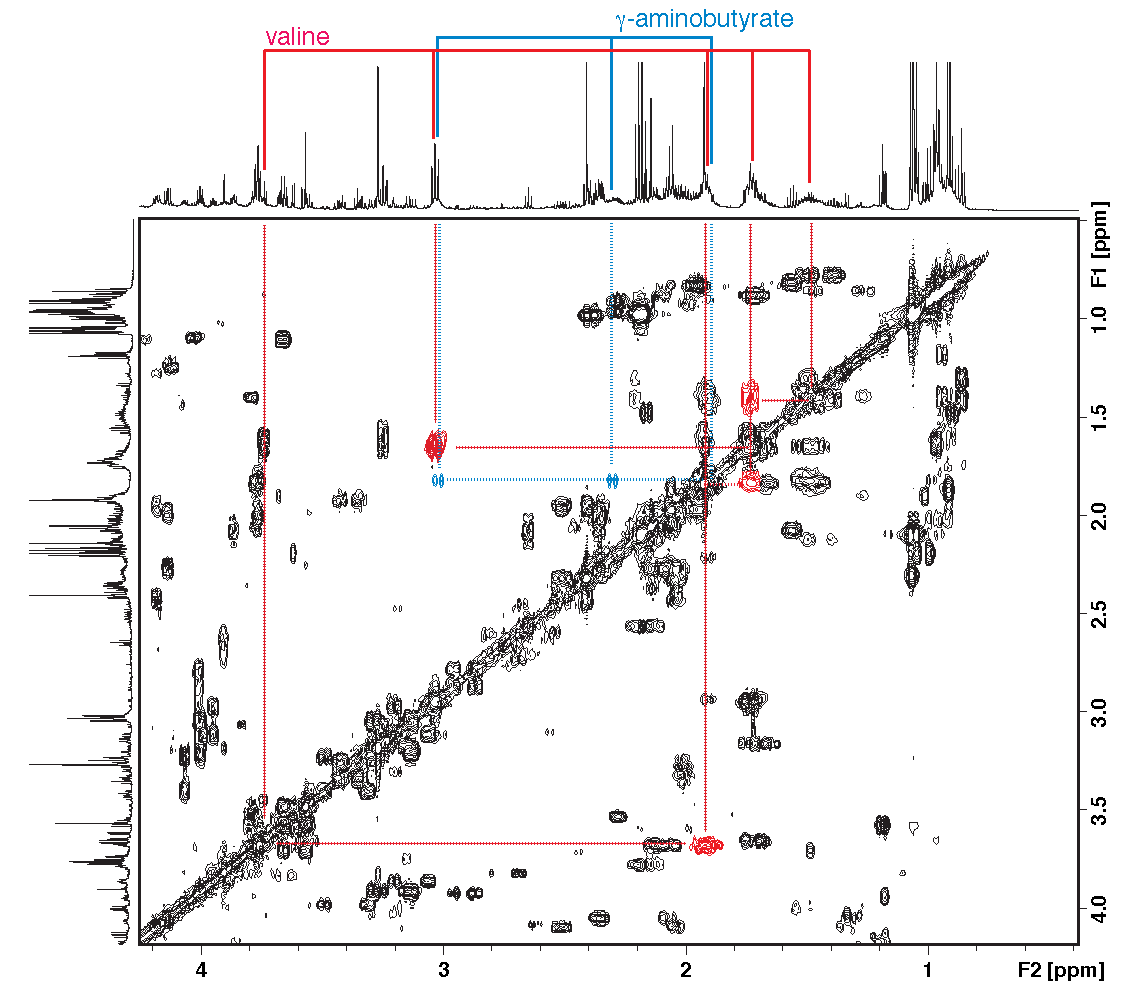
\includegraphics[width=0.8\textwidth]{ch2_figS5}
\caption[2D $^1\!$H NMR spectra collected on a single sample of supernatant from co-culture of \textit{Clostridium} ASF356 and \textit{Parabacteroides} ASF519]{\textbf{2D $^1\!$H NMR spectra collected on a single sample of supernatant from co-culture of \textit{Clostridium} ASF356 and \textit{Parabacteroides} ASF519} 2D spectra show gamma-aminobutyrate, not 5-aminovalerate, in the region overlapping with valine in 1D. Peaks corresponding to valine shown in red, gamma-aminobutyrate shown in blue.}
\end{figure*}

We also tested the effect of concurrent supplementation with Stickland pairs \textit{in silico}, which did not lead to any predicted growth benefit because the GENREs do not contain Stickland fermentation reactions. Stickland reactions are absent from reaction databases used to construct and curate GENREs such as the ModelSEED biochemistry database \cite{Henry2010-um}, but are present in the AGORA resource of semi-automatically generated GENREs for gut microbes \cite{Magnusdottir2017-dk}. None of the genes involved in Stickland fermentation have been identified in the genome of \textit{Clostridium} ASF356 as of this writing (determined via searching the annotated \textit{Clostridium} ASF356 genome in PATRIC \cite{Wattam2017-tk}, BLAST against D-proline reductase gene subunits). Taken together, these results suggest that proline and alanine co-supplementation confers a growth benefit through an alternative pathway or through Stickland fermentation with subsequent breakdown of 5-aminovalerate.

\section{Discussion}

In this study, we used data-driven methods to identify metabolic signatures that may contribute growth modulation in bacterial co-cultures, proposed mechanisms by which a specific signature may arise, and verified that growth of the benefiting strain is enhanced when putatively-crossfed metabolites are supplemented \textit{in vitro}. The biochemical capability we evaluated experimentally, Stickland fermentation of proline and alanine, is widely distributed in proteolytic \textit{Clostridia} \cite{Mead1971-oa}. While the ability of species inhabiting the mammalian gut to perform Stickland fermentation has been investigated, this study connects possible Stickland fermentation to a metabolic interspecies interaction that modulates growth. Given that some of the end products of Stickland fermentation were present at low concentrations in the fresh medium, and that \textit{Parabacteroides} ASF519 consumed them in monoculture (isobutyrate, isovalerate, and isocaproate), our data suggest that this interaction may be bidirectional. This observation supports some theoretical motifs for metabolism in the gastrointestinal tract proposed in the literature, such as the model of carbon and nitrogen flow proposed by Fischbach and Sonnenburg in which \textit{Clostridia} (e.g. \textit{Clostridium} ASF356) ferment amino acids, providing ammonium and other amino acid fermentation products to \textit{Bacteroides} (e.g. \textit{Parabacteroides} ASF519, which was assigned to the genus Bacteroides prior to 2006) \cite{Fischbach2011-wg,Sakamoto2006-oz}. \textit{Clostridium} ASF356 and \textit{Parabacteroides} ASF519 are co-located along the mouse gastrointestinal tract, however the relevance of this observation is unclear given a microbiota as restricted in size as the ASF \cite{Sarma-Rupavtarm2004-jv}. This kind of interaction has direct relevance to enteric pathogens, as emerging evidence indicates that in vivo utilization of proline via Stickland fermentation is highly active in \textit{Clostridium difficile} during sustained infection in mice \cite{Fletcher2018-ws,Jenior2017-lv,Jenior2017-zv}.

We expect that the growth outcome observed in the co-culture of \textit{Clostridium} ASF356 and \textit{Parabacteroides} ASF519 is due to a multitude of interactions that each have a small effect. An alternative mechanism by which co-culture could enhance growth is consumption of growth-inhibiting metabolite products. Although we did not explore them in this study, ConYE identified several cases in which this process may have occurred. For example, in the co-culture of \textit{Lactobacillus} ASF361 and \textit{Parabacteroides} ASF519, lactate, hypoxanthine, AMP, and UMP were all metabolites produced by \textit{Lactobacillus} ASF361 and consumed by \textit{Parabacteroides} ASF519 that were less abundant than expected in co-culture. Of these metabolites, lactate is known to have potent antimicrobial properties both broadly and against \textit{Lactobacillus spp.}\cite{Shelef1994-lb}, thus it is a reasonable candidate for this mechanism.

We developed ConYE to interrogate growth-modulating interactions within this study, but the framework can be used to study interspecies interactions that alter other phenotypes of interest. For example, the same analyses conducted here could be performed using consumption of a substrate of interest, such as lactose, to calculate metabolite yields as a function of that substrate rather than as a function of strain abundance. In this scenario, ConYE could be used to identify co-culture pairings that enhance conversion of lactose to a metabolite of interest, and identify cross-fed metabolites that contribute to enhanced yield of that metabolite of interest.

There is increasing interest in developing methods for inference of growth or abundance-modulating interactions between microbes from various data types and environments \cite{Friedman2017-zn,Weiss2016-tq,Xiao2017-yl}. These methods have primarily been focused on discovering interspecies interactions and the role they might play in ecosystem function, rather than ascribing mechanism to those interactions. Interspecies interactions are likely to be highly context-dependent, so more detailed knowledge about mechanisms of interaction is necessary to generalize these findings \cite{Chamberlain2014-nt}. Several approaches that integrate the metabolic and/or spatial environment using genome-scale metabolic models have been developed that account for context dependency \cite{Chan2017-tk,Harcombe2014-ev,Zomorrodi2012-ja}. However, limitations in biochemical knowledge across the bacterial tree of life limit their broad application to other organisms. Large-scale efforts to collect and assimilate biochemical knowledge of gut microbes within genome-scale metabolic models are in progress, but experimental data to validate and improve the predictive ability of these models is lacking \cite{Magnusdottir2017-dk}. Recent work to determine defined growth conditions for gut microbes will accelerate the process of experimental validation for such models, but data are still extremely sparse relative to organisms for which highly predictive metabolic models have been developed \cite{Tramontano2018-xz}. Similar metabolic model-based approaches have been applied to simplified versions of communities such as the human gut microbiota \cite{Bauer2017-kf,Chan2017-tk}, but the poor experimental tractability of these systems makes testing predicted interspecies interactions challenging and thus they are left unvalidated.

Incorporating dynamic substrate utilization information may be able to provide more accurate insight into metabolic interactions than the method we present. We envision that our method may be used as an efficient screening step in which many species are grown across many media conditions to identify putative interactions. Then, in conditions with many putative interactions, sampling can be performed with finer time resolution to attain a clearer picture of the actual coupling of metabolite consumption and production with changes in growth of individual species, as previously performed with yeast and lactic-acid bacteria \cite{Ponomarova2017-ob}. This framework, and others that model substrate utilization within a microbial community over time, could be modified with the strain abundance normalization procedure used within ConYE to identify dynamic features of emergent metabolic behavior in these communities \cite{Erbilgin2017-la}.

We have developed an experimental and computational pipeline to probe interspecies interactions and infer putative metabolic mechanisms of interaction, generating testable hypotheses.  Understanding mechanisms of interspecies interaction and the environmental conditions that induce them is a prerequisite to engineering communities with specific therapeutic or industrial value. For generalizable methods that predict interspecies interaction using mechanistic models to be successful, methods must be validated experimentally. This task will require a substantially larger set of observed interspecies interactions than are presented here, or are available in the literature, from which to derive generalizable principles. Extending our approach and similar methods to defined communities across conditions that are more diverse, both in terms of resource availability and spatial structure, will begin to make predictive modeling of interspecies interactions tractable.

\section{Methods}
\subsubsection{Strain maintenance}

All strains are identified within the manuscript by their genus followed by the original isolate designation numbers for the ASF, and solely by their designation numbers within figures. Formal designations as shown in \textbf{Figure 2.1B} are as follows: \textit{Clostridium sp.} ASF356, \textit{Lactobacillus intestinalis} ASF360, \textit{Lactobacillus murinus} ASF361, \textit{Eubacterium plexicaudatum} ASF492, \textit{Pseudoflavonifractor sp.} ASF500, and \textit{Parabacteroides goldsteinii} ASF519. \textit{Mucispirillum schaedleri} ASF457 was excluded from the study due to lack of detectable growth in the experimental medium, and \textit{Clostridium sp.} ASF502 was excluded due to inconsistent growth in the experimental medium. Stock vials for all ASF strains were maintained at -80°C in 50\% glycerol, 50\% brain-heart infusion (BHI) medium (see media formulations for the composition of brain-heart infusion media used in this study). All strains were grown in an anaerobic chamber (Shellab BACTRONEZ, Sheldon Manufacturing, Inc., Cornelius, Oregon, USA) filled with mixed anaerobic gas (5\% CO2, 5\% H2, 90\% N2). Anaerobic conditions were ensured through the use of palladium catalysts (baked at 120°C when outside the chamber and rotated daily when first entering the chamber) and anaerobic indicator strips (Oxoid, Basingstoke, UK).

\subsubsection{Media formulation}

Supplemented Brain–Heart Infusion medium, referred to as BHI throughout the manuscript: Brain–Heart Infusion base (37g/L, BD, Franklin Lakes, NJ, USA), supplemented with yeast extract (5 g/L), 0.2mL of vitamin K1 solution (0.5\% vitamin K1 dissolved in 99.5\% ethanol), 0.5mL/L of hemin solution (0.5 g/L dissolved in 1\% NaOH, 99\% deionized water), L-cysteine (0.5 g/L) and 5mL/L each of newborn calf serum, horse serum, and sheep serum. Vitamin K1, hemin, and all sera were added after autoclaving the medium. For preparation of agar plates, agar was supplemented at 12g/L.

Modified Lennox LB medium, referred to as mLB throughout the manuscript:  30g/L LB base in powder form (Sigma, St Louis, MO, USA) was combined with 0.376g/L L-cysteine (Sigma), 39mL of a mineral salts solution (containing 6g/L KH2PO4, 6g/L (NH4)2SO4, 12g/L NaCl, 2.5g/L MgSO4•7H2O, 1.6g/L CaCl2•2H2O, all dissolved in deionized water), 15mL/L of hemin solution (0.5 g/L dissolved in 1\% NaOH, 99\% deionized water), 0.3mL of vitamin K1 solution (0.5\% vitamin K1 dissolved in 99.5\% ethanol), 15mL/L of lactose solution (5g/L lactose dissolved in deionized water) and 15mL/L of tween 20 solution (1g/L tween 20 dissolved in deionized water).

All supplements that were made using deionized water, or those that could not be autoclaved, were filter-sterilized using a 0.22{\textmu}m membrane (except the sera).

\subsubsection{\textit{In vitro} monoculture and co-culture growth experiments in 12-well plates}

Strains were inoculated from frozen stock to grow a dense lawn on agar plates containing BHI media. Prior to inoculation, all agar plates were equilibrated inside an anaerobic chamber for at least 24 hours. Inoculated plates were incubated for 3-9 days before being used to start overnight cultures. For overnight cultures, 50mL of mLB broth in a 500mL glass flask was inoculated using a generous streak from the lawn of each strain, then each flask was covered with a Breathe-Easy membrane (Diversified Biotech, Dedham, Massachusetts, USA). After 18-24 hours of incubation at 37°C, overnight cultures were transferred to 50mL conical tubes, sealed, transferred out of the chamber, and centrifuged at 1500 xg for 5 minutes. After centrifugation, samples were transferred into the chamber, supernatant was poured off, and pellets were resuspended in 12.7mL mLB broth. The resuspension for each species was then diluted to make inoculant with the same concentration of cells as a solution at an optical density of 0.01, measured at OD600 with 100{\textmu}L of sample volume in a flat-bottom 96-well plate (with a well diameter of 0.64cm) using a Tecan infinite m200 plate reader (Tecan Group Ltd., Männedorf, Switzerland). This final inoculant was then used to inoculate mLB broth in 12-well plates. For monoculture samples, 100{\textmu}L of inoculant was added to 2.9mL of media. For co-culture samples, 100{\textmu}L of each strain’s inoculant was added to 2.8mL of media. 12-well plates were covered with a Breathe-Easy membrane, then the 12-well plate lid was placed on top of the membrane. Inoculated, covered 12-well plates were incubated at 37°C for 72 hours.

After 72 hours of incubation, 12-well plates were removed from the incubator and membranes were opened for each well using a razor. For each well, the sample was mixed by pipetting 900{\textmu}L three times, then 1.8 mL of sample was transferred to a 2mL snap-cap tube. 200{\textmu}L of sample was also collected after mixing and transferred to a 96-well plate to measure optical density at OD600. Samples within 2mL tubes were then transferred out of the chamber and centrifuged at 18407 xg for 2 minutes. After centrifugation, supernatant was poured directly into a 3mL syringe attached to a syringe pump filter (0.22{\textmu}m pore size, mixed cellulose ester filter) and filtered into a 2mL snap-cap tube. Cell pellets were then resuspended in 400{\textmu}L Qiagen lysis buffer (Buffer ASL, Qiagen) and vortexed until thoroughly mixed. Resuspended pellets and spent media were then frozen at -80°C.

To ensure reproducibility, 3 experiments were performed in which independent overnight starter cultures were used to inoculate 3 samples per monoculture and co-culture condition (resulting in 9 total replicates). For the third experiment, \textit{Eubacterium} ASF492 and \textit{Pseudoflavonifractor} ASF500 did not appear to grow in monoculture according to both OD600 and qPCR, and their metabolomes did not appear significantly different than any negative controls, so all sample groups containing \textit{Eubacterium} ASF492 and \textit{Pseudoflavonifractor} ASF500 in the third experiment were excluded from analyses. As a result, those sample groups have N = 6 replicates throughout the study.

\subsubsection{\textit{In vitro} amino acid supplementation experiments}

Inoculant for \textit{Clostridium} ASF356 was prepared as described for monoculture and co-culture experiments in 12-well plates. Solutions of amino acids in deionized water were filter-sterilized (0.22{\textmu}m pore size) and transferred to the anaerobic chamber and allowed to equilibrate for one week. Equilibrated solutions were mixed with liquid mLB broth (prepared as described previously), generating solutions that contained 90\% mLB and 10\% supplement by volume. Final concentrations were 1.25g/L for single amino acid supplements and 1.25g/L of each of two amino acids for supplements containing two amino acids (i.e. individual amino acids are at the same concentration in supplements containing one or two amino acids). 96-well plates were filled with 193{\textmu}L media and 7{\textmu}L inoculant (approximately the same initial density as in 12-well experiments), covered with a Breathe-Easy membrane, then incubated at 37°C for 72 hours. After incubation, the 96-well plates were removed from the anaerobic chamber, the breatheasy membrane was peeled off each plate, and the OD600 was measured in the 96 well plate.

\subsubsection{DNA extraction}

Zirconia beads (1mm; BioSpec Products) were added to samples in ASL buffer (QIAmp Stool kit), and samples disrupted using a Mini-Beadbeater (15s, two times), followed by heat treatment (5 min, 90°C, 800rpm; Eppendorf Thermomixer). Debris was pelleted (14,000 xg, 1 min), and 400{\textmu}L transferred to a QIAcube rotor adapter. Total DNA from each sample isolated on the QIAcube using the ‘human stool’ protocol provided by the manufacturer and stored at -20°C prior to PCR. Purified DNA used for standards in PCR assays was quantified using the DeNovix dsDNA kit. DNA standards were adjusted to 2ng/{\textmu}L and diluted 10-fold to generate standard curves in PCR assays.

\subsubsection{Hydrolysis probe-based qPCR assay design}
4-plex (including \textit{Clostridium} ASF356, \textit{Eubacterium} ASF492, \textit{Clostridium} ASF502, and \textit{Parabacteroides} ASF519) and 3-plex (\textit{Lactobacillus} ASF360, \textit{Lactobacillus} ASF361, and \textit{Pseudoflavonifractor} ASF500) hydrolysis probe-based quantitative polymerase chain reaction (qPCR) assays were designed to quantify the abundance of each strain’s DNA with high specificity and throughput \cite{Holland1991-gw}. Probe and primer design began with the \textit{groEL} gene, which encodes the highly-conserved molecular chaperone GroEL, as a putative target. The National Center for Biotechnology Information PrimerBLAST web interface was used to identify PCR targets for each strain with minimal sequence similarity with any region in another strain’s genome \cite{Ye2012-eb}. PCR products ranging from 70-200 base pairs with a calculated melting temperature between 57°C and 63°C were determined, requiring at least two mismatches with unintended targets, with at least two mismatches occurring within the last five base pairs at the 3’ end. We screened the top three primer pairs for each strain returned by PrimerBLAST for sensitivity and specificity using standard SYBR green chemistry, and determined that all primers for \textit{Lactobacillus} ASF360, \textit{Lactobacillus} ASF361, and \textit{Pseudoflavonifractor} ASF500 had poor sensitivity. To identify alternative PCR products for \textit{Lactobacillus} ASF360, \textit{Lactobacillus} ASF361, and \textit{Pseudoflavonifractor} ASF500, we performed BLAST for each putative gene in each strain against all other putative genes in ASF strains. For genes with no off-target hits (E-value \textgreater\! 1.0 for all comparisons), we attempted primer design using PrimerBLAST until a gene was found for each strain with at least 4 suitable primer pairs. All 4 primer pairs for the remaining ASF strains were screened for specificity and sensitivity and at least one suitable primer pair was found for each strain.

For all 7 strains in the qPCR assays, probes were then designed for each primer pair. The 7 strains were split into a 3-plex and 4-plex reaction based on typical density observed experimentally, with strains growing to higher densities in the 4-plex reaction and strains growing to lower densities in the 3-plex reaction. For each probe in each reaction, we performed multiple sequence alignment using Clustal Omega \cite{Sievers2011-bk}. Suitable probe sequences were identified manually according to five criteria: 1) maximize the number of mismatches at the 5’ end of the probe, 2) probe length between 20-30 base pairs, 3) estimated melting temperature around 66-70°C, 4) 35-65\% GC content, and 5) no G or C at the 5’ end of the probe. Final primers, products, probe sequences, and accompanying probe fluorophores and quenchers are provided in Table S1. Since only relative comparisons within each strain are made, the effects of non-single copy genes do not confound the data.

Primers and probes were synthesized by Integrated DNA Technologies, Inc. (Coralville, Iowa, USA). PerfeCTa 5X MultiPlex qPCR ToughMix (Quantabio, Beverly, MA) was used for all reactions. Each PCR reaction (20{\textmu}L total volume) contained ToughMix (1X concentration), 300nM of each forward primer, 300nM of each reverse primer, and 100nM of each probe, with 4{\textmu}L of DNA sample. The optimal cycling conditions were determined to be: initial denaturation of 3min @ 95°C followed by 40 cycles of 15s @  95°C and 30s @  61°C. All assays achieved an efficiency between 91.4\% and 100.5\%, except for Cy5 quantification in the first and third of 3 total 96-well plates used in the study. These assays achieved an efficiency of 124.4\% and 138.8\%, respectively. Efficiency was calculated using a diluted DNA standard (10-fold dilution starting with 2ng/{\textmu}L down to 0.002 ng/{\textmu}L) for each strain created using purified genomic DNA. Each PCR plate contained independent standard curves. Reactions were run using the BioRad CFX Touch, and analyzed using the software provided (where Cq value is equated to DNA concentration based on the standard curve).

Throughout the manuscript, qPCR data are presented as abundance values for each strain, which are z-score normalized using the mean monoculture abundance to center the data (i.e. mean value from each strain’s monoculture corresponds to a z-score of 0) and the standard deviation of monoculture abundance to scale the data. Thus, the z-score for the abundance of a strain can be compared across any condition. Abundance of every strain was quantified in all samples (including negative controls), and cross-contamination was not detected in any sample.

\subsubsection{Mono- and co-culture growth curve experiments}

Inoculant was prepared as described for 12-well experiments, wells were inoculated using the same starting cell density as used in 12-well experiments, and identical growth conditions were used. Optical density was measured at 589nm using a miniaturized plate reader \cite{Jensen2015-mw}. Experiments were performed in 96 well plates with 200{\textmu}L total volume in each well and a breatheasy membrane. Each sample group (monocultures and co-cultures) contains 8 biological replicates from a single experiment (e.g. each replicate was grown in an independent well, but they were derived from the same starter culture). After 72 hours, samples were removed from the anaerobic chamber, the breatheasy membrane was removed, and the endpoint optical density was recorded in a Tecan Infinite m200 plate reader (Tecan Group Ltd, Männedorf, Switzerland) at OD600. This endpoint optical density was used to linearly scale the values from the miniaturized plate reader. Raw and scaled growth curve data are available in the github repository accompanying the paper.

\subsubsection{$^1\!$H nuclear magnetic resonance spectroscopy-based metabolomics}

Samples were prepared for $^1\!$H NMR spectroscopy as described by Dona et al. \cite{Dona2014-og}. Samples were thawed at room temperature and centrifuged at 12000 xg at 4°C for 10 minutes, before 540 {\textmu}L of supernatant was combined with 60 {\textmu}L of buffer (pH 7.4; 1.5mM KH2PO4, 0.1\% TSP (3-(trimethylsilyl)propionic- 2,2,3,3-d4 acid sodium salt) in 100\% D2O) and transferred to a SampleJet NMR tube (Bruker BioSpin, Rheinstetten, Germany). Standard one-dimensional (1D) $^1\!$H-NMR spectra with water pre-saturation were acquired at 300 K using a 600 MHz Avance III spectrometer (Bruker), equipped with a SampleJet autosampler (Bruker). A total of 32 scans were collected into 64000 data points for each sample. Spectra were automatically phased, baseline corrected and calibrated to the TSP resonance at {\textdelta}1H 0 in Topspin 3.1 software (Bruker). The spectra were imported into MATLAB R2014a (The Mathworks, Inc., Natick, MA, USA). Biologically irrelevant regions of the spectra were removed (TSP resonance at {\textdelta}$^1\!$H 0 and residual water peak {\textdelta} $^1\!$H 4.5- 5.2) before peak alignment by recursive segment-wise peak alignment (RSPA) \cite{Veselkov2009-ha}. The loadings of pairwise principal component analysis models, as well as manual comparisons between fresh media spectra and spent media of each bacterial strain, were used to assign metabolite identities to peaks. To further identify metabolites that may only have been produced or consumed in co-culture, group means for all 15 co-culture conditions were compared to fresh media across the entire spectra. The relevant regions of the spectra were integrated to calculate relative spectral intensities for each metabolite. Metabolite identities were assigned by reference to known spectra in multiple databases. For all analyses, integrals were centered by subtracting the mean value for each metabolite in the blank samples, then scaled by the maximum absolute value of all centered values (so that the minimum and maximum possible scaled values for each metabolite were -1 and +1, respectively). We assume that concentration is proportional to the integrated peak area for each metabolite across all samples, thus relative concentrations can be inferred for each metabolite across all samples. After 72 hours of growth in this medium, pH ranges from 5.48-6.55 for these strains, thus only minor pH-dependent effects may be present in the spectra. The peak integral values, scaled values, peak integration regions and identities, and associated R code for analysis and visualization is available in the github repository. Raw spectra are available in the Metabolights database under identifier MTBLS705 \cite{Kale2016-aa}.

Additional two-dimensional (2D) NMR experiments ($^1\!$H-$^1\!$H correlation spectroscopy [COSY]) were performed on a selected sample of supernatant from co-culture of \textit{Clostridium} ASF356 and \textit{Parabacteroides} ASF519 to assist with metabolite identification \cite{Beckonert2007-cj}. For these experiments a total of 512 increments with 4 scans were acquired into 2 k data points with a spectral width of 12 ppm for each dimension.

\subsubsection{Differential abundance testing}

DNA quantification data for each sample group (each strain in monoculture and each unique co-culture condition) were tested for normality using the Shapiro-Wilk test (implemented via the shapiro.test function in R version 3.4.2) \cite{Royston1982-mm}. The data for all but one monoculture sample groups were normally distributed, but the majority of co-culture sample groups were non-normally distributed, so the non-parametric Mann-Whitney U-test was chosen to test for differential DNA abundance. The same procedure was performed for the metabolomic data, and the majority of sample groups and metabolites were found to be non-normally distributed, so the Mann-Whitney U-test was performed to test for differential metabolite abundance as well, identifying metabolites as either produced, consumed, or unchanged based on testing results and the value of the group mean relative to the fresh media. For tests of differential abundance, the false discovery rate (FDR) was controlled using the Benjamini-Hochberg procedure \cite{Benjamini1995-nd}. For DNA differential abundance testing, the number of sample groups used for FDR control was 21 (6 monocultures and 15 co-cultures). For metabolite differential abundance testing, the number of sample groups used for FDR control was 1806 (21 mono- and co-culture groups, each with 86 integrated metabolite peaks that were tested for differential abundance against fresh media samples). The results of all normality and differential abundance testing, and notebooks performing the calculations, are available in the github repository accompanying this work.

\subsubsection{Principal Component Analysis (PCA)}

PCA was performed on integrated peak values using the PCA function implemented in sci-kit learn (v0.19.2) in python v3.6 \cite{Pedregosa2011-wa}.

\subsubsection{Constant Yield Expectation (ConYE) model}

For each sample group, metabolite integrals were centered by subtracting the mean value of the metabolite integral in fresh medium (i.e. negative control). Centered integrals were then scaled by the max of the absolute values across all sample groups for each metabolite, resulting in values for each metabolite being scaled between -1 and +1, with at least one sample group taking a value of -1 or +1 for each metabolite. For each monoculture sample group, the mean of each scaled, centered metabolite was then divided by the mean DNA abundance of the corresponding strain, resulting in a metabolite yield specifying the amount of increase or decrease of a metabolite per unit of DNA for each strain. For each co-culture sample, the expected concentration of each metabolite was determined by multiplying the abundance of each strain in co-culture by the monoculture-derived yield, summing the two quantities from each strain, then subtracting the concentration of the metabolite in the fresh medium using the mean across negative controls (N=9). Using the calculated expected concentration from all samples within a co-culture group, deviation from expectation was determined by comparing expected concentrations to the observed concentrations in co-culture. Differential abundance was determined using the Mann-Whitney U-test with FDR control via the Benjamini-Hochberg procedure \cite{Benjamini1995-nd} and the mean of differences between expected and observed concentrations was recorded. The sample size used for FDR control was 1290 (15 co-culture groups, each compared to a simulated ConYE value for each of 86 metabolites). We explored the effect of variation in metabolite yields by leave-two-out bootstrap sampling of monocultures when performing the average yield calculation, followed by completion of the rest of ConYE for each subsample, and did not find that the results of significance testing were influenced by this subsampling (\textbf{Figure 2.9}). Jupyter notebooks performing the calculations for ConYE, the results of all tests, and the exploration of yield bootstrapping are available in the github repository accompanying this work.

\begin{figure*}[tb]
\centering
\includegraphics[width=0.8\textwidth]{ch2_figS4}
\caption[Selected examples of ConYE results using bootstrapped strain abundances.]{\textbf{Selected examples of ConYE results using bootstrapped strain abundances.} Top row shows the distribution of ConYE \textit{p}-values for each metabolite and bottom row shows the distribution of difference from the expected value for the same metabolite within each column. Examples are from the co-culture of \textit{Clostridium} ASF356 and \textit{Parabacteroides} ASF519. Distributions were generated by recalculating the average abundance of each strain in monoculture using leave-two-out bootstrapped samples prior to calculating the monoculture yield for each metabolite. N=50 samples with replacement for each monoculture.}
\end{figure*}

\subsubsection{Draft genome-scale metabolic network reconstruction and analysis}

Draft genome-scale metabolic network reconstructions (GENREs) were generated for \textit{Clostridium} ASF356, \textit{Lactobacillus} ASF360, \textit{Lactobacillus} ASF361, \textit{Eubacterium} ASF492, \textit{Pseudoflavonifractor} ASF500, \textit{Clostridium} ASF502 (not included in the present study), and \textit{Parabacteroides} ASF519 using a local installation of ProbModelSEED \cite{Benedict2014-yo,Henry2010-um}. Draft genome sequences for the strains from the same experimental stock used in this study were used as input to ProbModelSEED \cite{Wannemuehler2014-cn}. Briefly, ProbModelSEED annotates the genome for each organism to identify metabolic functions associated with genes or sets of genes. This process results in a draft GENRE containing high-confidence reactions for each species. To enable biomass production in the GENRE, gapfilling is performed with uptake enabled for any metabolite with a transporter annotated in the draft GENRE (i.e. simulating a rich medium). The resulting GENRE contains the original reactions associated with the organism’s annotated genome, as well as non-gene associated reactions added to enable biomass production. ProbModelSEED also assigns reaction probabilities to each reaction that can be added during gapfilling, which are derived using sequence similarity for genes which did not meet the similarity threshold for annotation via RAST, or reactions for which portions of a complex were not detected. These probabilities are incorporated during gapfilling, leading to preferential addition of reactions for which there was some genetic evidence.

\subsubsection{Metabolomics-constrained gapfilling}

After generation of draft GENREs, we added functionality to the GENREs using a previously-generated supernatant metabolomics dataset in which the same ASF strains were grown in the same medium used in this study \cite{Biggs2017-fs}. Using the original metabolite annotations for the dataset, we constrained the GENRE for each ASF strain by forcing production and consumption of any metabolite with a z-score normalized abundance of \textgreater\! +1 or \textless\! -1, respectively. Z-scores from the publication from which the data were drawn were used. This constraint was enforced by setting the lower bound of the exchange reaction for produced metabolites to 0.001 mmol/(g dry weight * hour), and the upper bound for exchange reactions for consumed metabolites to -0.001 mmol/(g dry weight * hour). The value of the constraint (0.001 mmol/(g dry weight * hour)) was chosen to be arbitrarily low, since absolute changes in metabolite concentrations were not derived in the metabolomics dataset used for gapfilling. Then, we set the remaining boundary conditions for each GENRE to represent the medium in which they were grown (as described in the \textit{in silico} simulations section), and forced arbitrarily low flux through the biomass reaction (0.005/hour). Then, we checked for transporters for each metabolite for each strain that enabled import (for consumed metabolites) and export (for produced metabolites). If a suitable transport reaction was not present, we added a transporter from the ModelSEED biochemistry database and constrained the directionality to be as observed (e.g. import only for consumed metabolites, export only for produced metabolites). Transporter assignments are provided in Table S2. We then performed gapfilling using a modified version of the SMILEY algorithm \cite{Reed2006-qv} as implemented in COBRApy v0.5.11. See “Metabolomics-constrained gapfilling” for exact algorithmic details. We used the set of all ProbModelSEED reactions for which reaction probabilities were assigned as the universal reactions for gapfilling, but excluded reactions containing O$^2$. We weighed the penalty for addition of each of these reactions by 1 - \textit{p}, where \textit{p} is the reaction probability, which ranges from 0 for unlikely reactions to 1 for highly likely reactions. The effect of this penalty is that high-probability reactions are assigned lower penalties, and are thus more likely to be added to the GENRE during gapfilling. For each ASF strain, metabolomics-constrained gapfilling was performed 10 times, each for 10 iterations, resulting in an ensemble of 100 GENREs. All 100 GENREs for each strain were unique (i.e. none of the iterations resulted in identical reaction sets being added to the draft GENRE).

\subsubsection{Metabolomics-constrained gapfilling algorithm}

Metabolomics-constrained gapfilling was performed to ensure the GENRE for each species could produce biomass in the in vitro medium and produce and consume metabolites as determined by supernatant metabolomics. We used a modified version of the SMILEY algorithm \cite{Reed2006-qv} with variable reaction penalties calculated in ProbModelSEED \cite{Benedict2014-yo}. We implemented and applied the modified version of our algorithm in COBRApy v0.5.11 \cite{Ebrahim2013-eb}. The algorithm is formally defined as:

\begin{equation*}
\begin{array}{rlll}
\min & \multicolumn{2}{l} {\sum c_{j}a_{j} } \\
\textrm{s.t.} &	Sv + Uy = 0	 \\
&	v_{biomass} \geq 0.005 hr^{-1} \\
&	v_{lb,i} \leq v_i \leq v_{ub,i}	& 	\forall i \in [1, N_s] \\
&	a_{j}y_{lb,j} \leq y_j \leq a_{j}y_{ub,j}	&	\forall j \in [1, N_u], a \in{[0,1]} \\
&	0.001 \leq v_k \leq v_{ub,j}	&	\forall k \in [1, N_k] \\
&	v_{lb,g} \leq v_g \leq -0.001	&	\forall g \in [1, N_g] \\
\end{array}
\end{equation*}

Where:
  $S$ is the stoichiometric matrix for the draft GEM;
	$U$ is the universal reaction library (as a stoichiometric matrix);
	$N_s$ and $N_u$ are the number of reactions in $S$ and $U$, respectively;
	$v$ is the vector of fluxes through $S$;
 	$y$ is the vector of fluxes through $U$;
	$v_{lb,i}$, $v_{ub,i}$, $y_{lb,j}$, and $y_{ub,j}$ are the lower and upper bounds on $v_i$ and $y_j$, respectively;
  $N_k$ and $N_g$ are the number of exchange reactions for metabolites that were produced and consumed, respectively;
	$v_{biomass}$ is the flux through the biomass reaction.
  $c = 1 - p$, where p is the probability of each reaction derived from ProbModelSeed
  $a$ is the integer indicator for each reaction in $U$

Biomass flux constraints and exchange reaction constraints were chosen to force arbitrarily-low activity through the corresponding reactions.

We performed gapfilling for 10 independent runs for each species, in which each run had 10 dependent iterations that each generate a solution containing a set of reactions that, when added to the GENRE and activated, satisfy the constraints (all metabolites can be produced and consumed as indicated, and biomass can be produced). Within each run, the penalty for each reaction was increased by setting  to encourage unique solutions. For reactions in the ModelSEED biochemistry that did not receive probabilities because they have no associated gene (e.g. spontaneous reactions), we set  to discourage addition of these reactions unless they were essential for any solution to be found. After each of 10 independent runs, reaction penalties were reset to their original value prior to beginning the next run. We reduced the integrality threshold in COBRApy to 1E-8 from the original value of 1E-6, because the default setting returned many solutions that did not satisfy the constraints applied due to numerical error for Lactobacillus ASF361 (e.g. the reaction list returned did not enable biomass production for this species because reactions from the universal reaction bag had values for  that were below 1E-6; decreasing the integrality threshold properly returned these reactions and anabled biomass production). For every ASF strain, all 100 GENREs constructed were unique.

\subsubsection{GENRE quality control}

All GENREs within the ensemble for each strain were assessed for mass balance. To perform this assessment, an intracellular demand reaction was added for each metabolite in the GENRE, and all exchange reactions were closed. Flux through each demand reaction was then optimized iteratively, and demand reactions that could carry flux indicated presence of a mass-imbalanced reaction that allowed spontaneous generation of the metabolite. This process identified three reactions in the draft GENREs that were mass-imbalanced (SEED ids: rxn15543 in \textit{Parabacteroides} ASF519 GENRE; rxn33894 and rxn30984 in \textit{Lactobacillus} ASF361). These reactions were removed from the draft GENREs, and the metabolomics-constrained gapfilling process was repeated using the draft GENREs with the reactions removed. These reactions have been removed from the ModelSEED biochemistry database since the generation of these draft GENREs.

All GENREs within the ensemble for each strain were also assessed for infeasible ATP production. Using boundary conditions that mimic the in vitro medium (as in in silico simulations, below), we optimized flux through an ATP demand reaction, and found that all GENREs for all strains generated between 0.5 and 1.9 mmol ATP/(g dry weight * hour). Normalizing this value by the uptake of lactose, which was 0.22 mmol/(g dry weight * hour) for all strains, gives a yield range of 2.27-8.64 units of ATP per unit of lactose, within reason for anaerobic organisms (for example, Escherichia coli is known to produce 2.2-3.2 units of ATP per unit of glucose when grown anaerobically) \cite{Muir1985-ft}. Although erroneous energy generating cycles may be present in the GENREs presented here, the realistic ATP yield determined for all GENREs suggests they are unlikely to influence simulation results in this media condition.

\subsubsection{\textit{In silico} simulations}

Flux balance analysis (FBA) was performed using version 0.8.1 of the COBRApy package \cite{Ebrahim2013-eb}. Ensembles of GENREs were analyzed using COBRApy methods through the Medusa package (See chapter 3 of this document, https://github.com/gregmedlock/Medusa/). Media composition was determined by calculating exact concentrations for defined supplements (Hemin, Vitamin K1, Lactose, Tween-20), and a concentration of 1mM was assumed to allow an uptake rate of 1 mmol/(g dry weight * hour). For media components with approximately known concentrations in LB (amino acids), the uptake rate was set to 5 mmol/(g dry weight * hour) based on a concentration of around 5 mM for most amino acids in LB \cite{Sezonov2007-hp}. For components detected via metabolomics that were not amino acids or supplemented, and therefore likely originated from the yeast extract in LB, the maximal uptake rate was set to 0.1mmol/(g dry weight * hour). For \textit{in silico} media supplements and knockouts, a metabolite was considered essential if removal of the metabolite from the in silico medium caused the flux through biomass to fall below 1E-5/hour (used because of limits of numerical precision for the solvers used; use of a lower threshold (1E-10/hr) does not affect these results).

\subsubsection{Data and software availability}

All raw and processed data and all code used in this project except software used to process raw NMR spectra are available at \url{https://github.com/gregmedlock/asf_interactions}. Where possible, Jupyter notebooks \cite{Kluyver2016-pl} are used for reproducibility and to display results alongside corresponding analyses. The raw NMR spectra have been deposited in Metabolights under MTBLS705.

\section{Acknowledgments}

We acknowledge the UVA ARCS staff for assistance setting up software used for gapfilling on the UVA computing cluster. We thank Jie Liu for helpful guidance on hydrolysis probe design for qPCR, and Thomas Moutinho for experimental assistance performing sample extraction. We thank all members of the Papin lab for helpful project feedback. We acknowledge funding from National Institutes of Health R01GM108501, T32LM012416, and T32GM008136.

\section{References}
\printbibliography[heading=none]


\section{Supplemental Figures}

\begin{suppfigure*}
\centering
\includegraphics[width=\textwidth]{ch2_figS1}
\caption[Heatmap describing supernatant metabolomes for all mono- and co-cultures after growth.]{\textbf{Heatmap describing supernatant metabolomes for all mono- and co-cultures after growth.} Red indicates higher concentration than fresh medium, while blue indicates lower concentration. Values are centered at 0 using the mean value in fresh media, then scaled between -1 and +1 by dividing by the maximum change in concentration for each metabolite in any sample in the study. Only metabolites for which an identity could be determined are shown. Hierarchical clustering of metabolites was performed using Euclidean distances and complete linkage.}
\end{suppfigure*}

\begin{suppfigure*}
\centering
\includegraphics[width=\textwidth]{ch2_figS2}
\caption[Optical density-based growth curves for \textit{Clostridium} ASF356, \textit{Lactobacillus} ASF360, \textit{Lactobacillus} ASF361, \textit{Eubacterium} ASF492, and \textit{Parabacteroides} ASF519.]{\textbf{Optical density-based growth curves for \textit{Clostridium} ASF356, \textit{Lactobacillus} ASF360, \textit{Lactobacillus} ASF361, \textit{Eubacterium} ASF492, and \textit{Parabacteroides} ASF519.} Optical density was measured at 589nm. Experiments were performed in 96 well plates with 200{\textmu}L total volume in each well. Each sample group (monocultures and co-cultures) contains 8 biological replicates from a single experiment (e.g. each replicate was grown in an independent well, but they were derived from the same starter culture). Line shows the mean for each sample group, and shading extends one standard deviation from the mean in both the positive and negative direction. Sky blue line indicates monoculture for the strain labelled in sky blue along the x axis. Orange line indicates monoculture for the strain labelled in orange along the y axis. Black line indicates co-culture of the two strains. Diagonal shows the monoculture growth curve for each species. Axes units are identical on all subplots. Time is shown in hours, extending to 72 hours.}
\end{suppfigure*}

\end{refsection}

%------------------------------------------------------------------------------------
% Chapter 3 Guiding the refinement of biochemical knowledgebases with ensembles of metabolic networks and machine learning
%------------------------------------------------------------------------------------
\chapter{Guiding Curation of Metabolic Networks with Ensembles and Machine Learning}
\chaptermark{Curation Guidance}
\begin{refsection}

The contents of this chapter are published as a preprint here:

\medskip\noindent
Medlock GL, JA Papin. (2018). Guiding the refinement of biochemical knowledgebases with ensembles of metabolic networks and semi-supervised learning. \textit{bioRxiv}, 2018. \url{https://doi.org/10.1101/460071}


\section{Context}

One of the initial goals of the work presented in the previous chapter was to develop genome-scale metabolic network reconstructions for the ASF strains and use them to predict growth-modulating interactions between strains in co-culture. As I become more knowledgeable about the true state of reconstructions for gut microbes and the amount of work and data that goes into most other reconstructions, I realized this goal could not be met in the near future. The primary issue was that metabolism for gut microbes, and the associated work on genetics, was underdeveloped relative to other organisms, so the reconstructions for gut microbes had an incredible number of gaps. For these reconstructions to make functional predictions, those gaps needed to be filled, but there was not sufficient publicly available data to decide how to fill those gaps. Matthew Biggs, another student in the lab, happened to be working on ensemble methods for construction and analysis of these reconstructions. The premise of this work was that we could probably make better decisions with these models if we accounted for multiple hypotheses when we needed to fill many gaps, as we did for gut microbes (e.g. account for all the ways to fill gaps in a network that make it functional, rather than a single way).

I performed some preliminary analyses with the reconstructions for the ASF species using ensemble modeling which took this one step further by applying machine learning to identify how these alternative gapfill solutions impacted co-culture simulations. The goal of this analysis was to identify targeted portions of the ASF reconstructions which we could manually curate to improve the certainty in the predictions we were making as much as possible. While this specific analysis will certainly be useful in the future to focus the massive amount of curation required for these networks, we still need to build substantial experimental capabilities with the ASF strains to derive much value from it. To demonstrate the value of this approach more generally, I reformulated it to refine predictions of gene essentiality, and applied it to organisms for which there was an abundance of publicly-available data. Thus, while the work in this chapter is primarily focused on bacteria that do not reside in the gut, we envision this approach being adopted for gut microbes such as the ASF strains.

Again, we have some terminology to clarify that may help the reader. In the constraint-based reconstruction and analysis (COBRA) field, researchers make clear distinctions between what they call \textbf{reconstructions} and \textbf{models}. A reconstruction can be thought of more as a database or knowledgebase; it is the systematic summary of the parts that make up an organism, which we choose to represent computationally. A model, in contrast, is a specific representation of an organism that can be used to simulate its behavior. Thus, reconstructions do not typically encompass information such as environmental conditions or biological objectives, whereas these may be explicitly represented in a model. Throughout this chapter, reconstructions are referenced as genome-scale metabolic network reconstructions (GENREs) and the models they are used to create are referenced as genome-scale metabolic models (GEMs).

\section{Synopsis}
Mechanistic models are becoming common in biology and medicine. These models are often more generalizable than data-driven models because they explicitly represent known interactions between components. While this generalizability has advantages, it also creates a dilemma: how should efforts be focused to improve model performance? We present an approach to this problem using ensembles of mechanistic models and machine learning, then apply it to genome-scale metabolic network reconstructions. We generate an ensemble of candidate models consistent with experimental data, then perform in silico simulations for which improved predictiveness is desired. We apply unsupervised and supervised learning to these simulation results to identify structural variation in ensemble members that maximally influences variance in simulation outcomes across the ensemble. These structural variants are high priority candidates for curation through targeted experimentation. We demonstrate this approach by applying it to 29 bacterial species to identify curation targets that improve gene essentiality predictions. Our approach represents a fully automated, scalable, and performance-driven recommendation system for curating hypothesis-driven models.

\section{Introduction}

Genome-scale metabolic network reconstructions (GENREs) are knowledgebases describing metabolic capabilities and their biochemical basis for entire organisms. GENREs can be mathematically formalized and combined with numerical representations of biological constraints and objectives to create genome-scale metabolic models (GEMs). These GEMs can be used to predict biological outcomes (e.g. gene essentiality, growth rate) given an environmental context (e.g. metabolite availability) \cite{Oberhardt2009-iu}. GEMs are now used widely for well-studied organisms such as Escherichia coli and Saccharomyces cerevisiae, but GEMs for most other organisms are much more taxing to create and curate, partially due to the exhaustive and manually-driven steps required \cite{Thiele2010-yq}.

Systems for automatically generating GEMs of sufficient quality for limited purposes have been developed \cite{Henry2010-um}, but the methods used to further curate GEMs are nearly universally under-reported in the literature. Curation methods for GEMs that take researchers many months to years to develop are often summarized qualitatively with limited description. This is not surprising, given the difficulty in prioritizing areas for curation of network-based, highly connected mechanistic models such as GEMs.

In practice, heuristics are typically used to prioritize curation, such as curating portions of the GEM directly involved in the manipulation of a metabolite, gene, or pathway of known interest. These heuristics, combined with targeted literature searches, allow task-based curation and GEM evaluation, which is increasingly supported in software related to genome-scale metabolic modeling \cite{Lieven2018-fo, Wang2018-yn}. However, identifying the network components that influence the predictions of interest is not an intuitive process because biological networks are generally highly connected.

One way to view this issue is through the lens of a sensitivity analysis, asking how much variation in the parameters of a model will impact a simulation of interest. Such an approach has been developed and applied to dynamic models of biological networks \cite{Babtie2014-vy}, which relies on quantified uncertainty in the structure of a model. Uncertainty quantification has been applied at the level of individual components within a GEM, either by considering the probability of a function being present in a network based on sequence comparisons \cite{Benedict2014-yo} or by leveraging network structure to more accurately estimate these probabilities \cite{Plata2012-ys}. However, an approach that unifies a probabilistic views of GEM structure with simulations performed with them, which would enable structural sensitivity analysis for GEMs, has not been developed to our knowledge.

\begin{figure*}[tb]
\centering
\includegraphics[width=\textwidth]{ch3_fig1}
\caption[ Approach for a simulation-guided recommendation system for curation of genome-scale metabolic models.]{\textbf{ Approach for a simulation-guided recommendation system for curation of genome-scale metabolic models.} \textbf{a)} A draft GEM is generated using ModelSEED. Algorithmic gapfilling is applied so that the GEM can recapitulate experimental observations, and the process is repeated to identify alternative solutions. These alternative solutions are assembled into an ensemble of GEMs, each of which contains the original content of the draft GEM and a unique set of gapfilled reactions. \textbf{b)} Single gene knockouts are performed using the ensemble, in which production of biomass is evaluated when reactions requiring each gene are inactivated. \textbf{c-d)} Machine learning approach for identifying curation targets based on ensemble simulations. Unsupervised machine learning is applied to the ensemble simulation results, generating two simulation clusters (cluster 1 [red] and cluster 2 [blue]). Here, principal coordinate analysis is used to visualize the similarity of simulation profiles for all models within an ensemble. Simulation clusters are then used as labels in supervised machine learning, which are predicted using model reaction content as input to a random forest classifier. Curation is prioritized based on the features contributing to classifier performance.}
\end{figure*}

Recently, we developed a framework for the generation of ensembles of GEMs which can be applied to improve predictive performance over that of an individual GEM \cite{Biggs2017-md}. This approach is analogous to the use of ensembles of data-driven models \cite{Dietterich2000-dq} or hypothesis-driven models such as signaling networks \cite{Kuepfer2007-gq}, and has been applied to metabolic networks for dynamic modeling as well \cite{Tran2008-pt}. Here, we extend our framework to prioritize curation of network-based biological models by coupling ensemble simulations with machine learning. One of the central tenets of systems biology is that models represent our hypotheses about how an organism functions. As such, we can use these models to simulate the behavior we expect according to our hypotheses. Our approach takes advantage of this, generating many hypotheses (e.g. an ensemble) and coupling them with machine learning to identify experiments that optimally improve our understanding of an organism.

\section{Results}

Our approach, which can be generalized to any mechanistic model and simulation task of interest, is summarized as follows. First, we generate many models that are each consistent with experimental data, forming an ensemble of models (\textbf{Figure 3.1a}). We then perform a set of simulations using the ensemble that are related to a task of interest, such as drug target identification or production of a metabolite of commercial interest (\textbf{Figure 3.1b}). Using the output of these simulations, we perform unsupervised learning to generate phenotypic clusters of models, where clustering is determined by similarity of simulation profiles across the entire set of simulations (\textbf{Figure 3.1c}). We then apply supervised learning to predict simulation cluster membership for each model using the values of variable parameters in that model as input (\textbf{Figure 3.1c}). The relative importance of these model parameters in the supervised learning model indicates the impact that uncertainty in that parameter has on simulation outcomes across the ensemble (\textbf{Figure 3.1d}). In other words, resolving the true state of these parameters will maximally reduce uncertainty in the simulations performed with the ensemble. Here, we apply this approach to the task of reducing uncertainty in predicted gene essentiality for 31 bacterial species (\textbf{Figure 3.1a-d}). We generate an ensemble for each species using previously published growth phenotyping data \cite{Plata2015-bc}, predict the effect of genome-wide single gene knockouts, then apply machine learning as described above.

\begin{figure*}[tb]
\centering
\includegraphics[width=\textwidth]{ch3_fig2}
\caption[ Subsampling of ensemble content and simulations to demonstrate exhaustive sampling of the solution space.]{\textbf{ Subsampling of ensemble content and simulations to demonstrate exhaustive sampling of the solution space.} \textbf{a)} The variable reaction content in ensemble members as a function of increasing ensemble size. A variable reaction is any reaction that has a variable state across any member of the subsampled group (e.g. it is off in some members and on in some members, but neither entirely off nor entirely on). For each species, the mean number of variable reactions in subsamples of GEMs is shown by the solid line, with the standard deviation shown as light fill of the same color above and below the mean. Subsampling was performed with 1000 draws per subsample size. Ensembles were sampled at intervals of 20 members, e.g. 20, 40, 60... until reaching the size of the entire ensemble. \textbf{b)} Variability in gene essentiality simulations within subsamples of ensemble members. Using the same subsampling procedure as in panel \textbf{a}, the number of genes with at least one GEM in the subsample with a simulation outcome different than the rest (e.g. non-consensus) was determined. The mean for each subsample size is shown by the solid line, with the standard deviation shown as light fill of the same color above and below the mean.}
\end{figure*}

\begin{figure*}
\centering
\includegraphics[width=\textwidth]{ch3_fig3}
\caption[ Application of the curation guidance pipeline to bacterial species.]{\textbf{ Application of the curation guidance pipeline to bacterial species.}  \textbf{a \& c)} Ensemble gene essentiality simulations and unsupervised learning for three representative species. Each heatmap displays essentiality simulations for each ensemble member (row label) after inactivating a single gene (column label). Black cells indicate genes predicted to be essential while white cells indicate genes predicted to be non-essential. Principal coordinate analysis (PCoA) plots next to each heatmap show the similarity between gene essentiality simulation profiles for each ensemble member. Within each PCoA plot, each point represents an ensemble member, colored by cluster membership as determined with k-means clustering (k=2). Percent variance in the pairwise distance matrix explained by each principal coordinate is indicated in parentheses. See Methods for analysis details. \textbf{b)} Example of a network feature driving simulation cluster membership. The top reaction, catalyzed by serine hydroxymethyltransferase, is the primary activity of the enzyme, which was annotated in the draft GEM. The bottom reaction is a promiscuous function of the same enzyme, which was the most important reaction in determining cluster membership (k=2) for \textit{Corynebacterium glutamicum}. (abbreviations; THF is tetrahydrofolate and 5,10-mTHF is 5,10-Methylenetetrahydrofolate). Water is excluded from reactants in the top reaction to simplify visualization. \textbf{d)} Evaluation of performance of GEMs in each simulation cluster compared to genome-wide gene essentiality data. Essentiality datasets from in vitro experiments were collected for \textit{Haemophilus influenzae} and \textit{Staphylococcus aureus}. Precision (TP/[TP + FP], TP = true positives, FP = false positives) and recall (TP/[TP+FN], FN = false negatives) were calculated for each ensemble member for each species. Small red and blue circles indicate an individual ensemble member, colored by simulation cluster membership. Large red and blue circles indicate mean behavior for ensemble members from each cluster, and error bars of same color extend above and below the mean by one standard deviation.}
\end{figure*}

Given our objective of identifying the most impactful experiment or curation effort to improve the quality of our models, we required that our ensembles were large enough to saturate the space of unique simulation results (i.e. predicted behavior) and model structures (i.e. hypotheses). Toward this end, we first subsampled the ensemble for each species and determined the unique reaction content within each subsample (\textbf{Figure 3.2a}). We found that unique reaction content plateaued or nearly plateaued with ensembles containing as few as 100-200 models, suggesting the ensembles we generated sufficiently saturate the space of unique reactions. In other applications, we suspect that organisms with lower quality GEMs (e.g. more gaps in their metabolic network) or less phenotypic profiling data may require additional sampling to saturate this space.

For gene essentiality simulations, the number of variable predictions (e.g. number of genes for which at least one ensemble member disagrees with another member) plateaued in a similar manner (\textbf{Figure 3.2b}). We also performed subsampling for predictions of genes essential for biomass production, which exhibited similar properties of convergence (\textbf{Supplemental Figure 3.1a-b}). Taken together, these subsampling-based results confirm that ensembles containing 1000 models generated using our reconstruction pipeline sufficiently represent the network structure space (e.g. unique reactions) and prediction space (e.g. essentiality profiles) possible given the input data. This behavior is consistent with our previous work examining the performance of ensembles of GEMs for Pseudomonas aeruginosa, in which various aspects of ensemble performance nearly plateaued with only 50 GEMs \cite{Biggs2017-md}. However, in order to ensure that an adequate number of samples are included for downstream machine learning analyses, we maintain the full ensemble of 1000 GEMs for each species in all analyses.

Each species’ ensemble contained 19.27 +/- 8.66 genes (mean +/- standard deviation) for which at least one GEM’s prediction of essentiality disagreed with another GEM in the ensemble, representing 3.11 +/- 1.39\% of total metabolic gene content. For the unsupervised machine learning portion of this analysis, we performed \textit{k}-means clustering on the gene essentiality simulations from each species’ ensemble separately. We chose \textit{k} = 2 to generate two clusters for each species, each of which contain GEMs from the ensemble with similar gene essentiality simulation profiles. The results are visualized for a subset of species using principal coordinate analysis (PCoA) in \textbf{Figure 3.3a} and \textbf{3c}. Although we chose \textit{k} = 2 here to illustrate our approach, the separation of models in PCoA space suggests that for many species, determining a larger number of clusters might be advantageous. For example, while \textit{k} = 2 generates two maximally-different simulation clusters, there may be more than two distinct \textit{in silico} phenotypic clusters that represent significant differences in hypothesized model behavior. Accounting for the presence of these smaller clusters may identify important network features that would otherwise only be found through multiple iterations of clustering with \textit{k} = 2 and refinement of the ensemble.

We next sought to identify the reactions that vary across an ensemble that are associated with membership in each cluster. For this objective, we trained a random forest classifier \cite{Breiman2001-pl} to predict cluster membership for each GEM from its reaction content. The classifier for every species had an out-of-bag accuracy above 97\%, indicating that gene essentiality cluster membership can easily be predicted from reaction content within the ensembles. To prioritize candidate reactions for curation of each species’ ensemble, we examined the features that contributed the most to classifier performance.

One way to resolve the identity of these prioritized reactions is a targeted literature search, which might reveal information that has not been incorporated into genomic or metabolic databases. For example, in the ensemble for \textit{Corynebacterium glutamicum}, the strongest driver of essentiality cluster membership was inclusion of the reaction L-threonine acetaldehyde-lyase, which converts L-threonine to glycine and acetaldehyde (\textbf{Figure 3.3b}). This activity is known to occur in \textit{C. glutamicum}, but was not annotated in its genome because the enzyme primarily uses L-serine as a substrate (serine hydroxymethyltransferase, \textbf{Figure 3.3b}), while conversion of L-threonine is considered a side activity \cite{Dong2011-wt,Simic2002-ia}. The correct function was present in 97 of the ensemble members in the blue cluster and 0 members of the red cluster, representing 84.3\% of the blue cluster. Given that these 97 models only represent 9.8\% of the entire ensemble for \textit{C. glutamicum}, this function would have been overlooked if ensemble features were chosen by consensus across the ensemble rather than via machine learning. This result highlights the ability of our approach to identify discrepancies between databases and the literature (such as under-annotated promiscuous enzyme activity) while also prioritizing investigation into these issues based on their contribution to prediction uncertainty.

Our approach is focused on prioritizing curation efforts to reduce uncertainty in model simulations. However, whether this approach generally improves the predictive performance of GEMs is unclear. To investigate this question, we evaluated the performance of a subset of ensembles for which experimental genome-wide gene essentiality datasets derived from in vitro growth on a rich medium were available. Suitable datasets were identified for \textit{Staphylococcus aureus} \cite{Chaudhuri2009-za} and \textit{Haemophilus influenzae} \cite{Akerley2002-ja}. Each GEM in the ensembles for these species was evaluated using precision (the ratio of true positives to the sum of true and false positives) and recall (the ratio of true positives to the sum of true positives and false negatives; \textbf{Figure 3.3d}). For both species, ensemble members had variable precision and recall, and simulation cluster membership is associated with a difference in both precision and recall (\textit{p} \textless\! 0.0001, Mann-Whitney U-test with false discovery rate control via Benjamini Hochberg procedure). Based on this result, selecting models for future analyses by excluding one of the two simulation clusters will improve performance as evaluated against experimental data. Thus, our curation guidance approach will improve model performance when the true state of a parameter is associated with the cluster with better performance.

\section{Discussion}

The analysis we performed demonstrates just one possible path towards the goal of reducing uncertainty in our understanding of biochemical networks within the framework we propose. Changes to the process can be rationalized for new goals; for example, we previously demonstrated that introducing random weights on inclusion of each reaction during algorithmic gapfilling can generate more diverse ensembles \cite{Biggs2017-md}. If none of the ensemble members generated by our pipeline adequately represented metabolism for an organism (e.g. their gene essentiality simulation results were vastly different than experimental observations), we could introduce such random variance to increase the likelihood of generating some ensemble members that reflect biological reality. Such an approach may be necessary for organisms with metabolic repertoires differing substantially from those represented in popular biochemical databases (e.g. gut microbes, intracellular parasites). Inclusion of methods for proposing novel hypothetical enzymatic function could complement our approach for such organisms \cite{Hatzimanikatis2005-wy,Jeffryes2015-bm}.

Our approach builds on work in other disciplines in which uncertainty quantification and reduction are applied to understand or improve the behavior of domain-specific models. For example, in petroleum engineering, a similar ensemble-based approach is used to derive value of information (VOI) estimates for resolving parameter values in models of oil reservoir management \cite{He2018-nb}. In the application of our framework demonstrated here, we effectively derive VOI estimates for resolving reaction presence or absence. Taking a VOI approach for biological discovery and to improve models used in various facets of biotechnology could help automate workflows and substantially reduce costs by prioritizing experiments. As the diversity and depth of organisms that mechanistic models such as GEMs are being constructed for increases, such approaches will be vital to continue to improve their quality and predictiveness \cite{Magnusdottir2017-dk,Monk2014-fa}.

\section{Methods}
\subsubsection{Organism selection}

Organisms with available growth phenotype data were extracted from Plata, et al. \cite{Plata2015-bc}. To identify a representative genome for each species, we queried the PATRIC database \cite{Wattam2017-tk} with the genus and species name for all organisms in the study, then selected a single genome from PATRIC based on decision criteria described as follows. When a reference genome was assigned for the species, the genome identifier for the reference genome was chosen. If no reference genome was available, a genome listed as “representative” was chosen. When multiple genomes with the “representative” status were available, we chose the first genome listed. If a selected representative genome contained more than 10 contigs, a representative genome with fewer contigs was chosen. Strain identifiers were not provided in the study from which data was drawn, so these selection criteria were developed to select the highest-quality genome available for the species in the study. Selected genome identifiers are available in \textbf{Supplemental Table S1}.

Organism selection was further refined by only including those from Plata, et al. which grew in at least 10 of the single-carbon source Biolog conditions. The experimental growth threshold originally used in the paper from which data were drawn was used (\textgreater\!10 colorimetric units of tetrazolium dye reduction; originally scaled between 0 and 100 based on positive [100 units] and negative [0 units] controls). This choice was made with the recognition that the tetrazolium dye measures redox activity and not actual biomass production; for the purpose of our study, we assume that detectable redox activity above 10 relative units would require biomass production. After this initial selection step, \textit{Brachybacterium faecium} and \textit{Gordonia bronchialis} were also removed from the analysis because no solutions existed to enable biomass production using the universal reaction bag for either species. \textit{Bacillus megaterium} was excluded because only one gapfill solution was found across all gapfilling cycles. Similarly, \textit{Stenotrophomonas maltophilia} was excluded because only two unique gapfill solutions were found. In total, the full analysis pipeline was applied to 29 species.

\subsubsection{Generation of draft genome-scale metabolic models}

Draft-quality genome-scale metabolic models (GEMs) were generated using the ModelSEED reconstruction pipeline \cite{Henry2010-um} accessed through PATRIC in August, 2018 \cite{Wattam2017-tk}. PATRIC servers were queried to generate GEMs formatted for use in COBRApy \cite{Ebrahim2013-eb} using the Mackinac package \cite{Mundy2017-eb}.

\subsubsection{Representative media}

The base medium for biolog conditions was derived from the ModelSEED media compositions for biolog plates. Flux variability analysis was used to identify metabolites which had essential uptake reactions in all complete media-gapfilled reconstructions from PATRIC. Based on this analysis, we added Heme and H\textsubscript{2}SO\textsubscript{3} to the base biolog composition used \textit{in silico} (i.e. uptake of heme and H\textsubscript{2}SO\textsubscript{3} was allowed in all conditions). For each single carbon source, appropriate identifiers were found in the ModelSEED database. For metabolites with ambiguous chemical identities (e.g. metabolites that Biolog does not provide isomer composition for, such as D-Galactose), only one isomer was selected from ModelSEED to represent the condition. Carbon sources that are complex mixtures of metabolites (gelatin) or polymers (pectin) were excluded from analyses.

\subsubsection{Algorithmic gapfilling}

Each individual gapfilling step, corresponding to enabling biomass production on a single media source, was performed using the following algorithm adapted from our previous work \cite{Biggs2017-md}. This algorithm is in essence the same as parsimonious flux balance analysis (pFBA, \cite{Lewis2010-xs}), except that the parsimonious assumption of minimization of the sum of all fluxes is only applied to reactions from a universal reaction bag that are activated to allow flux through the network. This algorithm takes the form:

\begin{equation*}
\begin{array}{rlll}
\min & \multicolumn{2}{l} {\sum abs(y_j) } \\
\textrm{s.t.} &	Sv + Uy = 0	 \\
&	v_{biomass} \geq 0.05 \\
&	v_{lb,i} \leq v_i \leq v_{ub,i}	& 	\forall i \in [1, N_s] \\
&	y_{lb,j} \leq y_j \leq y_{ub,j}	&	\forall j \in [1, N_u] \\
\end{array}
\end{equation*}

Where:
  $S$ is the stoichiometric matrix for the draft GEM;
	$U$ is the universal reaction library (as a stoichiometric matrix);
	$N_s$ and $N_u$ are the number of reactions in $S$ and $U$, respectively;
	$v$ is the vector of fluxes through $S$;
 	$y$ is the vector of fluxes through $U$;
	$v_{lb,i}$, $v_{ub,i}$, $y_{lb,j}$, and $y_{ub,j}$ are the lower and upper bounds on $v_i$ and $y_j$, respectively;
	$v_{biomass}$ is the flux through the biomass reaction.

The formulation is identical to the original formulation of pFBA, except for four key differences. First, we only require an arbitrarily low amount of flux through biomass, rather than the maximum amount of biomass, meant to represent a binary growth condition. Second, we introduce a universal reaction bag ($U$) and associated flux variables $y$ for each reaction in $U$. Third, only fluxes through reactions in $U$ are penalized; fluxes through reactions in the model being gapfilled ($S$) are not penalized. Fourth, rather than explicitly splitting all reactions into irreversible reactions, we take advantage of solver-level interfaces implemented in COBRApy through the optlang package \cite{Jensen2016-nu} that allow introduction of absolute values into the objective (this is done out of convenience in our implementation; this aspect of the problem formulation is identical to the same aspect in pFBA at the solver level). As in Biggs et al. , the solution to this optimization problem activates reactions in the universal reaction bag with the minimum sum of fluxes necessary to enable flux through the biomass reaction in a given condition \cite{Biggs2017-md}.

\subsubsection{Generating ensembles from gapfill solutions}

For each organism, the entire algorithm for generating an ensemble is Described in \textbf{Algorithm 1}.

\begin{algorithm}
  \caption{Iterative gapfilling}
  \begin{algorithmic}[1]
    \For{\texttt{$i$ in [0,1,...,N]}}
      \State $\mbox{randomly order a selection of $J$ conditions}$
      \For{\texttt{each condition $j$ in $J$}}
        \State $\mbox{Set medium for $j$}$
        \State $\mbox{Gapfill}$
        \State $\mbox{Add gapfilled reactions}$
      \EndFor
      \State $\mbox{Store solutions}$
      \State $\mbox{reset reaction penalties}$
    \EndFor
  \end{algorithmic}
\end{algorithm}

We performed this procedure for 1000 cycles for each species (i.e. N = 1000). After completing the procedure, the solutions from each iteration (e.g. $[1,2,...,N]$) are each converted into an ensemble member. All species included in the study grew in at least 10 \textit{in vitro} single carbon source media conditions (i.e. $J$ contained at least 10 conditions); for each species, all positive growth conditions were used to gapfill during each cycle. After removing duplicate gapfill solutions, all species included for further analyses had 970-1000 members in their ensemble (species not considered after this point are detailed in \textit{Organism selection}). See \textbf{Figure 4.4} in \textbf{Chapter 4} for a graphical description of this algorithm.

\subsubsection{Ensemble flux balance analysis and ensemble gene essentiality}

Ensemble flux balance analysis and ensemble gene essentiality screens were performed using Medusa v0.1.2 (unpublished, see Chapter 4 and https://github.com/gregmedlock/Medusa) and COBRApy v0.13 \cite{Ebrahim2013-eb}. The GNU linear programming kit (GLPK) was used as the numerical solver in all cases. For all simulations, rich medium was used (1,000 mmol/gram dry weight*hr uptake allowed for all metabolites with a transport reaction; commonly referred to as “complete medium”). An arbitrarily low cutoff for flux through biomass in gene essentiality screens was used (1E-6 units of biomass/hr), but varying this quantity between 1E-10 and 1E-3 did not substantially affect essentiality results.

\subsubsection{Subsampling of ensemble features and predictions}

For all subsampling performed, 1,000 random draws were made with replacement at each subsample ensemble size. Ensemble sizes for each subsampled population ranged from 20 to 1,000, with subsampling performed in intervals of 20 members (i.e. 20, 40, 60, ... 1,000 members). When the subsample size exceeded the actual ensemble size (e.g. some species had slightly less than 1,000 members), all ensemble members were subsampled.

\subsubsection{Clustering of ensemble gene essentiality predictions and prediction of clusters}

Ensemble gene essentiality predictions were clustered into two clusters using \textit{k}-means clustering as implemented in the KMeans class of scikit-learn v0.19.2 \cite{Pedregosa2011-wa} (max iterations=300, convergence tolerance=1E-4, Elkan’s \cite{Elkan2003-du} algorithm). Gene essentiality predictions were converted to binary data (essential or nonessential) using a cutoff of flux through biomass of 1E-6 mmol/(gDW*hr). Random forest classification was performed to predict cluster membership using active features in each ensemble member (e.g. presence or absence of a reaction was assigned as True or False in the input, respectively) \cite{Breiman2001-pl}. The RandomForestClassifier class from scikit-learn v0.19.2 was used (500 trees, quality of splits determined with the gini criterion, no max depth, minimum of 2 samples per split, minimum of 1 sample per leaf, the square root of the number of features searched at each split, training samples determined for each tree via bootstrap selection with replacement). The default metric in scikit-learn’s RandomForestClassifier for determining feature importance, the mean decrease in node purity, was used to calculate feature importance in this study \cite{Gordon1984-iw}.

\subsubsection{Visualization of gene essentiality clusters}

Principal coordinate analysis (PCoA) \cite{Gower1966-xt} was used to visualize ensemble gene essentiality results. PCoA as implemented in scikit-bio v0.5.4 (\url{https://github.com/biocore/scikit-bio}) was performed using the hamming distance \cite{Hamming1950-zv} to compute the pairwise distance matrix.

\subsubsection{Gene essentiality datasets}

Gene essentiality datasets were identified for species in this study from the Online Database of Gene Essentiality (OGEE, \cite{Chen2017-cs}). In cases where multiple datasets were available for a given species, the dataset generated using the same strain of the species selected for GENRE reconstruction was selected. If multiple datasets still existed for a species, a single dataset was chosen based on media richness (e.g. more complex media were selected over simpler media). We excluded the essentiality dataset for \textit{Streptococcus pneumoniae} because the total set of screened genes was not included \cite{Song2005-uc}. In brief, the authors developed a kanamycin insertion cassette targeted for 693 genes that were selected based having \textgreater\!40\% amino acid sequence identity with a set of well-studied organisms. The authors reported the identity of only the essential genes, so non-essential genes that would be in the dataset could not be included in our set of predictions. Based on these selection criteria and limitations, we selected datasets from OGEE for \textit{Staphylococcus aureus} \cite{Chaudhuri2009-za} and \textit{Haemophilus influenzae} \cite{Akerley2002-ja}.

\subsubsection{Data and analysis availability}

All data, analysis scripts, results, and models generated are available at \url{https://github.com/gregmedlock/ssl_ensembles} and will be archived on Zenodo upon acceptance for publication after peer review. Archived results include the analysis pipeline results for all species in the study (rather than only the representative examples shown here).

\section{Acknowledgements}

We acknowledge funding from National Institutes of Health R01GM108501, T32LM012416, the Thomas F. and Kate Miller Jeffress Memorial Trust, and a Wagner predoctoral fellowship to GLM. We thank Matthew Biggs for thoughtful discussion related to the manuscript and Maureen Carey for helpful comments on drafts.

\section{References}

\printbibliography[heading=none]

\section{Supplemental Figures}

\begin{suppfigure*}
\centering
\includegraphics[width=\textwidth]{ch3_figS1}
\caption[ Subsampled ensemble behavior for predictions of biomass production.]{\textbf{ Subsampled ensemble behavior for predictions of biomass production.} We simulated biomass production in a rich medium across the entire ensemble and subsampled these results at varying ensemble sizes. \textbf{a)} Standard deviation of the mean flux through biomass from each subsample and \textbf{b)} standard deviation of the standard deviation of flux through biomass in each subsample. For both quantities (variance of the mean of each subsample and variance of the variance of each subsample), simulations plateau before inclusion of all 1000 ensemble members. Values on y axis are normalized by dividing by the mean flux through biomass for the entire ensemble.}
\end{suppfigure*}

\end{refsection}

%------------------------------------------------------------------------------------
% Chapter 4 Software for analysis and generation of ensembles of genome-scale metabolic network reconstructions
%------------------------------------------------------------------------------------
\chapter{Software for Ensemble Analysis of Metabolic Networks}
\chaptermark{Ensemble Modeling}
\begin{refsection}

The contents of this chapter will be submitted as a software article to PLoS Computational Biology as:

\medskip\noindent
Medlock GL, JA Papin. Building and analyzing ensembles of genome-scale metabolic network reconstructions using Medusa.

\section{Context}

Ensemble modeling has become ubiquitous in machine learning in recent decades, and nascent applications are starting to appear across areas of science that tend to use mechanistic (rather than data-driven) models. Working with relatively uncharacterized organisms such as the ASF strains, I found the new processes that thinking with ensembles allowed to be incredibly appealing. At the same time, Jason was also getting inquiries from other groups about these ensemble methods in response to Matt's paper on ensemble flux balance analysis, thus it seemed that there was broader interest. I wanted to use ensemble methods in the future, and could imagine a career heavily focused on integrating ensemble methods in systems biology. So, I decided that I would turn my efforts in graduate school into an open-source software package. This package, Medusa, is intended as a community-driven effort within the constraint-based reconstruction and analysis (COBRA) field. The entirety of the work in \textbf{Chapter 3} of this dissertation was performed in Medusa and has been recycled to be a core component of the Medusa documentation.

Software intended to share COBRA methods began being developed in the late 2000s, the largest efforts of which revolved around the MATLAB-based COBRA Toolbox. This tool is still actively developed, but a much larger ecosystem has developed as open-source software has permeated science. COBRApy is an open-source Python package for COBRA analyses that is part of this new ecosystem. I have become a frequent user and active contributor to COBRApy during my PhD. Working with and contributing to such packages, one quickly realizes how powerful community-driven development in this context can be. It allows for standardization of analyses, data, and a chassis on which new methods can be developed much more quickly than if they need to be implemented from the ground up. I benefited tremendously from COBRApy development, both the code and the community, during my PhD. The work in this chapter represents my attempt at creating a new ecosystem within this community, which I hope will have a mutualistic relationship with it for years to come.

As a note to the reader, this chapter is organized using the formatting style of Software articles, intended for submission to \textit{PloS Computational Biology}. This format is intended to communicate the structure and capability of the software, rather than focusing on the details of results that can be obtained with it. \textbf{Chapter 3} relied on this software, and further use cases and examples are available (and in development) in the Medusa documentation at \url{https://medusa.readthedocs.io/en/latest/}.

\section{Synopsis}

Uncertainty in the structure and parameters of networks is ubiquitous across computational biology. In constraint-based reconstruction and analysis of metabolic networks, this uncertainty is present both during the reconstruction of networks and in simulations performed with them. Here, we present Medusa, a python package for the generation and analysis of ensembles of genome-scale metabolic network reconstructions. Medusa builds on the COBRApy package for constraint-based reconstruction and analysis by compressing a set of models into a compact ensemble object, providing functions for the generation of ensembles using experimental data, and extending constraint-based analyses to ensemble scale. We demonstrate how Medusa can be used for ensemble simulations and how machine learning can be used in conjunction with Medusa to guide the curation of genome-scale metabolic network reconstructions. Medusa is available under the permissive MIT license from the Python Packaging Index (\url{https://pypi.org/}) and from github (\url{https://github.com/gregmedlock/Medusa/}), and comprehensive documentation is available at \url{https://medusa.readthedocs.io/en/latest/}.

\section{Introduction}

Hypothesis-driven computational models of biological systems are being increasingly applied to guide experimentation \cite{Kitano2002-az}. In hypothesis-driven modeling (also known as mechanistic modeling), hypothesized biological parts and interactions are mathematically formalized to allow in silico experimentation. These models take many forms, ranging in complexity from a single linear equation relating two quantities to dynamic systems of non-linear differential equations.

A unifying principle across all hypothesis-driven modeling frameworks is that the choice of model scope and parameter values may strongly influence simulation results. For some types of models, approaches from other fields have been applied to quantify the influence of parameter values on simulation outcomes, such as sensitivity analysis of dynamical models \cite{Marino2008-jt}. For network-based models of biological systems such as metabolic or signaling networks, the presence or absence of a network component may be uncertain due to lack of characterization or uncertainty in data itself. Traditional sensitivity analysis methods have recently been reformulated for these systems to analyze sensitivity to topological variation, but these methods have not seen wide adoption \cite{Babtie2014-vy}. While uncertainty in network structure poses analytic difficulties, it also presents an actionable framework to accelerate biological discovery. Alternative network structures can guide experimental design, whereby simulation results for alternative networks are each compared to experimental results to identify the network structure most consistent with biological behavior \cite{Medlock2018-kx,Silk2014-rv}.

In studies of metabolism, genome-scale metabolic network reconstructions (GENREs) have emerged as a useful formalism for hypothesis-driven modeling \cite{Oberhardt2009-iu}. In conjunction with biological objective functions, such as maximization of growth rate, GENREs can be used to construct genome-scale metabolic models (GEMs). In addition to topological uncertainty (e.g. presence/absence of reactions in a network), simulations with GEMs generally yield many alternative solutions. Even the simplest simulations that can be performed with GEMs exhibit this phenomenon. This is the case for flux balance analysis (FBA), in which a pseudo-steady state is assumed, and flux values are found for all reactions in a GEM such that an objective function is optimized \cite{Orth2010-kl}. When this convex optimization problem is solved, a global maximum for the objective function is guaranteed to be found. However, while a single maximum value for the objective is found, flux through every other component of the network is only constrained within a solution space, not to a single value. As a result, even though performing FBA yields a single value for the flux through reactions in a network, there are an infinite number of feasible flux values within the range determined by the solution space for some reactions. Techniques such as flux variability analysis and flux sampling have been developed to explore the space of alternative solutions in this scenario \cite{Mahadevan2003-ah,Schellenberger2009-bj}.

A myriad of additional algorithms have been developed for the analysis of GEMs for strain engineering, contextualization of experimental data, and building cell- and tissue-type specific GEMs \cite{Blazier2012-oo,Machado2014-wi,Wang2017-sp}. In addition to optimization problems that can be solved using linear programming such as FBA, problems have been formulated to take advantage of mixed integer linear programming (MILP). MILP employs binary state variables during optimization to solve problems that involve discrete activation or inactivation of variables. MILP problems are particularly well-suited to network-based models, since they allow switch-like behavior that can include or exclude network components (e.g. shutting reactions off/on). MILP has been used widely for gap-filling of GEMs, a process in which constraints or objectives are set to recapitulate a known phenotype by adding biochemical functions from a universal set of reactions \cite{Reed2006-qv}. In MILP problems used for gap-filling, the objective function is generally minimization of the number of modifications to a GEM that must be made to satisfy the constraints imposed (e.g. metabolite uptake or secretion, production of biomass). One consequence of this formulation is that alternative solutions, which contain unique sets of reactions which need to be altered in the network or added, are extremely common for large networks that have a large space of potential solutions to draw from (e.g. a large universal set of reactions). These alternative optima in MILP problems are increasingly being considered and leveraged to understand redundancy in solutions and whether or not portions of a solution may be spurious \cite{Karp2018-hd,Robaina-Estevez2017-fy,Rossell2013-cf}.

Previous work in our lab recently demonstrated that the order in which separate instances of gap-filling are applied to the same network (e.g. gap-filling for growth on individual carbon sources iteratively) strongly influences which reactions are included in the resulting network \cite{Biggs2017-md}. In this same study, the alternative solutions generated during this process were used to improve gene essentiality predictions using EnsembleFBA, a technique in which sets of alternative GEMs are used to perform FBA to determine gene essentiality. Using the entire ensemble, performance can be tuned by varying the voting threshold required to make a specific prediction, analogous to the threshold-based voting procedure used to construct receiver operating characteristic curves for ensemble-based machine learning models such as random forest \cite{Breiman2001-pl}. This approach is likely to be highly beneficial for studies of organisms for which little biochemical data are available, which typically have many gaps in their GENRE and thus have many highly-variable alternative gap-filling solutions. Although a nascent approach for studying GENREs, we have built on these observations, and ensemble generation and analysis have been applied for multiple use cases \cite{Machado2018-cz,Medlock2018-ub,Medlock2018-kx}.

Here, we present Medusa, a python package for the generation and analysis of ensembles of GENREs. Medusa provides a framework for compactly representing ensembles of GENREs, avoiding the redundancy of storing many separate models while still being flexible enough to allow variation in any component within a GENRE. Medusa manages ensemble storage and indexing during simulation, allowing users to interact with an entire ensemble in the same way they would interact with an individual GENRE using any constraint-based reconstruction and analysis (COBRA) method. Furthermore, by standardizing the representation of ensembles and their interface with existing COBRA methods, Medusa enables the application of supervised and unsupervised machine learning to gain insight into the influence of varying components within an ensemble of GENREs on the predictions they make. The architecture and functionality of Medusa make ensemble analyses as accessible and usable as COBRA methods applied to single networks.


\section{Design and Implementation}
\subsubsection{Architecture overview and dependencies}

Medusa is built on top of COBRApy, a Python-based package in which many COBRA methods are implemented \cite{Ebrahim2013-eb}. Although a dependency-free approach in which ensemble simulation methods are implemented from the ground up may be more efficient, we chose to extend COBRApy to greatly decrease the size and complexity of the codebase and to reduce the domain-specific knowledge required to use Medusa and understand the source code (i.e. decrease the effort for existing COBRApy users and contributors). As such, the architecture of Medusa closely mimics COBRApy (\textbf{Figure 4.1}).

At the time of this writing, GENREs are represented within COBRApy using a Model class. The Model class manages the interface between COBRApy and numerical solvers through optlang, a python package for formulating and solving optimization problems that extends the symbolic mathematics package SymPy \cite{Jensen2016-nu,Meurer2017-mu}. GENREs are represented by a Model using additional classes with biological analogs (Metabolite, Reaction, and Gene). In Medusa, ensemble functionality is introduced using 3 new classes. The first, Feature, describes a GENRE component which has a parameter that varies across an ensemble (e.g. a reaction that is reversible in some ensemble members but irreversible in others). The second, Member, describes individual GENREs within an ensemble and their state for each Feature. The third is the Ensemble class, which references all Features and Members associated with an ensemble of GENREs, as well as a COBRApy Model, referred to as the “base model”. This base model holds all COBRApy objects that might be associated with any member of the ensemble. Within an Ensemble, each Feature references the component within the base model (Metabolite, Reaction, or Gene) for which it encodes alternative parameter values, as well as the appropriate attribute within that component that is modified (e.g. the upper bound of flux through a reaction). When a simulation is to be performed using a particular GENRE within an ensemble, Medusa changes the state of the base model to represent the proper state for that ensemble member for every Feature. Thus, the Ensemble object can represent any number of variations in GENRE structure throughout an ensemble (e.g. reaction presence/absence, reversibility, alternative gene-protein-reaction relationships) and can be used to apply any methods implemented in COBRApy. Furthermore, this implementation has a memory footprint only slightly larger than a single COBRApy Model, and facilitates queuing of simulations for parallel processing.

Medusa is developed partially with test-driven development. Tests are implemented using the pytest package (\url{https://docs.pytest.org/en/latest/}) and tests are run automatically with each modification to the Medusa github repository via continuous integration with TravisCI (Travis CI, GMBH, Berlin, Germany). Support is provided for Python version 3.0 and later.

\begin{figure}[tb]
\centering
\includegraphics[width=0.9\linewidth]{ch4_fig1}
\caption[ Architecture of ensembles in Medusa.]{\textbf{ Architecture of ensembles in Medusa.} Ensemble functionality is implemented in Medusa through the Ensemble class. The Ensemble class exposes three attributes to the user: features, members, and base\_model. Both features and members are container-like objects similar to genes, reactions, and metabolites in COBRApy. Within each container, Medusa objects of class Feature and Member are stored. The base\_model attribute points to a COBRApy Model. This base\_model contains all of the features present in any member of the ensemble, and is manipulated when generating an ensemble or performing simulations.}
\end{figure}

\section{Results}
\subsubsection{Performing ensemble simulations}


Currently, users can perform FBA, flux variability analysis (FVA), single gene deletions, and single reaction deletions using an ensemble in Medusa. In each case, the simulations are performed with a single function, which returns a collection of results, where each entry corresponds to the simulation results for a single ensemble member. For the currently implemented analyses, the collection of results are returned as a pandas DataFrame, where each column corresponds to the entry normally populating the results for a single network (e.g. a reaction ID for FBA/FVA, a gene ID for single gene deletions), and each row corresponds to an ensemble member (except for FVA, where two columns are required for each ensemble member to describe the minimum and maximum). See \textbf{Figure 4.2} for a schematic describing how the shape of data describing simulation results changes for each simulation method.

\begin{figure}[tb]
\centering
\includegraphics[width=\linewidth]{ch4_fig2}
\caption[ Description and shape of simulation results for common COBRA methods as implemented in Medusa.]{\textbf{ Description and shape of simulation results for common COBRA methods as implemented in Medusa.} Each simulation method returns a distribution-equivalent to the single-model simulation result.}
\end{figure}

\begin{figure*}[tb]
\centering
\includegraphics[width=\textwidth]{ch4_fig3}
\caption[ Comparison of ensemble flux balance analysis (FBA) simulations across different conditions (A) and before and after ensemble-guided curation (B).]{\textbf{ Comparison of ensemble flux balance analysis (FBA) simulations across different conditions (A) and before and after ensemble-guided curation (B).} \textbf{A)} Ensemble FBA performed on glucose or mannose minimal media using an ensemble of 1000 GEMs for \textit{Staphylococcus aureus}. Mean for the distribution for either condition shown by vertical line of same color. Predicted flux through biomass is higher on mannose than glucose (Mann-Whitney U-test, \textit{p} \textless\! 0.05). \textbf{B)} Ensemble FBA performed on complete medium (uptake of -1000 mmol/g*DW*hr allowed for all metabolites) using an ensemble of 1000 GEMs for \textit{S. aureus}. Mean for the distributions before and after curation shown by vertical line of same color. Ensemble and machine-learning guided curation identified N-Formimino-L-glutamate iminohydrolase as a driver of variation in simulated flux through biomass. Based on a literature search, this reaction was inactivated in all ensemble members and ensemble FBA was performed again, resulting in the shift in the distribution shown. See documentation for full narrative-style example: \url{https://medusa.readthedocs.io/en/latest/machine_learning.html}.}
\end{figure*}


Because the Ensemble object implemented in Medusa maintains a COBRApy Model object, users can also perform any custom simulation they would like by 1) manipulating the COBRApy model to be suitable for their simulations (e.g. set custom constraints or objectives), 2) setting the state of the model to represent an ensemble member using Medusa functionality, 3) performing their simulation, then 4) iterating through any other ensemble members they would like and performing steps 2-3.

\subsubsection{Comparing ensemble simulations}

When performing simulations with an ensemble rather than a single model, results shift from single values to distributions. While this explicitly accounts for uncertainty, it also requires that statistical approaches are applied to interpret differences in distributions. In the simplest case, performing ensemble FBA to predict growth rate on each of two different media conditions for a single bacterial species generates two distributions of predicted growth rates (\textbf{Figure 4.3A}). A univariate test (e.g. t-test or a non-parametric equivalent) can be used to determine whether the predicted growth rate is equal in these two conditions. This example is demonstrated in full in the Medusa documentation at \url{https://medusa.readthedocs.io/en/latest/stats_compare.html}.

\subsubsection{Coupling ensemble models and simulations with machine learning}

The availability of ensemble generation and simulation methods in Medusa provides ample opportunity to apply machine learning to leverage variation in ensembles. One application area that we have developed focuses on guiding the curation of genome-scale metabolic network reconstructions by attributing simulation uncertainty to network components in the ensemble, then prioritizing curation of these components based on how much they contribute to simulation uncertainty \cite{Medlock2018-kx}. This approach can be broken down into three steps: 1) ensemble generation, 2) ensemble simulations, 3) unsupervised learning to summarize simulation uncertainty, and 4) supervised learning to associate uncertainty in network structure with uncertainty in simulations. In addition to our published work utilizing Medusa for this purpose, we provide an example in the Medusa documentation that applies this method to a single ensemble FBA simulation: \url{https://medusa.readthedocs.io/en/latest/machine_learning.html}).

In this example, a previously generated ensemble is loaded into Medusa, media conditions are set to allow uptake of any metabolites with transporters in the ensemble, and ensemble FBA is performed. Then, a random forest regressor is used to predict the simulated values for flux through biomass (e.g. the values generated with ensemble FBA) for each ensemble member using the Medusa states for the same ensemble member as input. Examining the most predictive feature in the random forest regressor, we perform a literature search which suggests that the feature is likely not present for the bacterial species under study. Based on this examination, we disable the feature (which is a reaction in this case), perform ensemble FBA again, and find that this curation step has reduced the average predicted flux through biomass (\textbf{Figure 4.3B}). Although we use this approach to guide curation, we also envision the same process having great utility for attributing simulation uncertainty more generically, such as with simulations performed using an ensemble generated using ‘omics integration methods \cite{Blazier2012-oo}.

\subsubsection{Generating ensembles from phenotypic data}

\begin{figure*}[!tb]
\centering
\includegraphics[width=0.9\textwidth]{ch4_fig4}
\caption[ Iterative gapfilling strategy used to generate ensembles implemented in Medusa.]{\textbf{ Iterative gapfilling strategy used to generate ensembles implemented in Medusa.}  \textbf{A)} Given a list of conditions in which an organism satisfied some objective (e.g. secretion of a specific metabolite, growth) and a draft GENRE for the organism, gapfilling is performed sequentially on each condition. After each gapfill step on a single condition, reactions in the gapfill solution are added to the GENRE before starting gapfilling on the next condition. In this schematic, all conditions are used, but Medusa also allows users to randomly subsample a fraction of conditions to generate more variation in the resulting gapfilled GENREs. Here, gapfilling is performed to enable growth in the presence of each individual metabolite (indicated by a green arrow for a single condition during each gapfill step). \textbf{B)} Medusa iteratively performs gapfilling as shown in panel \textbf{A}, then shuffles the order of conditions to introduce variation in the gapfill solution. After a user-defined number of cycles through the process shown in panel \textbf{A}, Medusa generates an ensemble containing all unique GENREs that resulted from gapfilling.}
\end{figure*}

Medusa implements a previously-developed algorithm for gapfilling GENREs using growth phenotyping data \cite{Biggs2017-md,Medlock2018-kx}. The algorithm takes a GENRE with an objective function and a dataset of binary growth/no-growth calls on defined media conditions as input. The objective function is then set as a constraint with bounds such that any feasible flux distribution must enable activity within the bounds (e.g. at least some amount of flux through biomass production or a demand reaction). A new objective function is set to minimize the sum of fluxes through reactions in the reaction database, and the problem is solved to identify reactions taking part in this minimal flux activity. To generate a single gapfilled ensemble member, the draft GENRE is iteratively gapfilled on each positive growth media condition. Variation is introduced by randomizing the order in which media conditions are used for gapfilling. See \textbf{Figure 4.4A-B} for a schematic summarizing this approach. This procedure is also summarized in \textbf{Chapter 3} in the methods section under \textit{Algorithmic gapfilling} and in \textbf{Algorithm 1} of the same chapter.

This gapfilling process is implemented in Medusa through a single function, and a full example of preparing a model and all data necessary for this process are provided in the Medusa documentation at \url{https://medusa.readthedocs.io/en/latest/creating_ensemble.html}. Although Medusa implements the previously published version of this approach, it also allows users to randomly subsample a fraction of conditions to generate more variation in the resulting gapfilled GENREs.

\section{Availability and Future Directions}

Stable releases of Medusa are available through the Python package index (PyPI, \url{https://pypi.org/}) as well as github (\url{https://github.com/gregmedlock/Medusa/}). Documentation is available through Readthedocs at \url{https://medusa.readthedocs.io}. Current development efforts are focused on parallelization and integrating Medusa with other python-based tools in the COBRA community.

Currently, the only high-level function available to users of Medusa to share ensembles generates a serialized version of the Ensemble object using the pickle package (the standard Python library package for serializing objects). Alternatively, users can save the base\_model for any Ensemble as a Systems Biology Markup Language (SBML, \cite{Hucka2003-io}) file using COBRApy, then choose the formatting option of their liking to save feature and member information for the ensemble. In SBML, there is not currently a standardized way to represent ensembles as required in Medusa. We plan on extending the Flux Balance Constraints package, an extension to SBML intended for constraint-based models, to enable standardized sharing of Medusa ensembles. Until then, we recommend users include both an SBML file for the base\_model of each Ensemble and the serialized pickle at time of publication.

\section{Acknowledgements}

We acknowledge funding from the National Institutes of Health R01GM108501, T32LM012416, the Thomas F. and Kate Miller Jeffress Memorial Trust, and a Wagner predoctoral fellowship to GLM. We thank members of the Papin lab for feedback on documentation and usability of Medusa.

\section{References}

\printbibliography[heading=none]
\end{refsection}

%------------------------------------------------------------------------------------
% Chapter 5 Reflections and Future Directions
%------------------------------------------------------------------------------------
\chapter{Reflections}
\begin{refsection}

Throughout this dissertation, I presented a new framework to infer metabolic interactions between microbes (\textbf{Aim 1}) and developed software and methods for the generation and analysis of ensembles of genome-scale metabolic network reconstructions (\textbf{Aim 2}). The work towards \textbf{Aim 1} will accelerate future efforts to understand metabolic interactions across multiple contexts not limited to the study of gut microbes. The work towards \textbf{Aim 2} provides much-needed infrastructure for researchers to perform ensemble simulations using genome-scale metabolic network reconstructions, as well as a framework for guiding curation of these reconstructions. Here, I detail the next steps which are enabled or inspired by this work, how this work fits into the broader fields that it relates to (microbiome research and systems biology), and my view on what research is necessary to advance these fields in the future.

\subsubsection{Future approaches to infer metabolic mechanisms of interspecies interaction}

Identifying the mechanisms that drive an association between two quantities or traits is a common problem in science. In microbiome studies, the associations we are frequently interested in are correlation between the abundance of two bacterial strains within the gut or correlation between the abundance of a bacterial strain and a disease phenotype in a host. In \textbf{Chapter 2}, we developed a data-driven approach to identifying metabolic mechanisms that might explain the interactions we observe between the abundances of two gut microbes grown \textit{in vitro}. This approach will be broadly applicable to other bacterial species, and we envision it being most useful for large screens to identify putative interactions, such as screening collections of microbes against a single pathogen to find conserved metabolic interactions that inhibit growth of the pathogen.

Alongside the data-driven approach we developed, we created genome-scale metabolic network reconstructions (GENREs) for the gut microbes we studied in \textbf{Chapter 2}. Thanks to the ensemble modeling methods we used, we saw that the predictions made using these models were highly uncertain, thus we interpreted simulations performed with them conservatively. This conservative interpretation, combined with insights from the data-driven modeling, pointed us in an interesting direction, and the follow-up experiments we performed confirmed that novel metabolic function was likely responsible for our observations. During this process, we used our GENREs to perform simulations that were analogous to the experiments we would perform to test findings from our data-driven modeling. This is an unconventional approach---generally, GENREs are used to exactly represent all or most of the experiments in a study, occasionally leading to very uncomfortable stretching of the assumptions required for the \textit{in silico} model to represent the \textit{in vitro} or \textit{in vivo} reality. We hope that in complex scenarios, such as the study of metabolic interactions amongst multiple organisms, researchers in the future are more willing to leverage GENREs to answer small questions well than to answer all-telling questions poorly.

Our work in Chapter 2 may be improved further given thoughtful collection of new data. One of the first improvements is primarily technical, and would be enabled by data with more replicates per condition and additional replicates collected in diverse, defined media conditions. In \textbf{Chapter 2}, we took an unpaired data analysis strategy to infer differentially abundant metabolites within the constant yield expectation (ConYE) framework. The data were treated as unpaired in the sense that metabolite abundances and strain abundances were averaged to calculate a yield value for each strain for each metabolite. However, it is possible to use the paired structure of the data to obtain an estimate of individual metabolite-level contributions to biomass production based in inter-replicate variability in the relationship between biomass and changes in metabolite concentration. We chose not to take this approach because of the complexity of the medium in the study, which might lead to many false positive inferences, e.g. many metabolites might be associated with small contributions to biomass production. Additionally, having only 6 replicates, with substantial variability in biomass across replicates, we were unlikely to have much power to detect these metabolite-biomass correlations.

To overcome these issues and enable this extension of ConYE, we will perform similar experiments using defined media recently developed for culturing gut microbes by another group, as well as additional replicates \cite{Tramontano2018-xz}. Furthermore, we will make use of the multiple defined media conditions developed in that work to build a data-driven, non-linear model that predicts strain population sizes based on metabolite consumption and production. We will use a non-linear model that allows for interaction between variables (e.g. abundance of each metabolite, in this case) which will identify redundant functions of media components (e.g. a particular amount of biomass is produced in the presence of metabolite A or metabolite B). This model could immediately be used to predict metabolic interactions between species that will affect growth, aiding the design of microbial communities for industrial purposes, or for the qualitative interpretation of data from other studies involving the strains for which the models were constructed. Alternatively, the same model could be used in a generative fashion within the same ConYE framework as in \textbf{Chapter 2}. Given strain abundances in co-culture, we could simulate expected metabolite abundances using the models constructed from monoculture data, then compare them to the observed metabolite abundances.

Another approach that could enhance future studies like those in \textbf{Chapter 2} involves pairing data-driven approaches like ConYE with hypothesis-driven models such as GENREs. In \textbf{Chapter 2}, we used ensembles of genome-scale metabolic models to evaluate the effect on growth in monoculture of individual metabolite supplements. These supplements were of interest because they may have been cross-fed according to the ConYE results, thus showing that the strain benefited from supplementation of the individual metabolite might support the inference. This approach was taken due to the highly uncertain model structure for each of the ASF strains, as well as the experimental difficulty of fully validating that cross-feeding occurred. Limited data are available to curate the genome-scale metabolic models for the ASF strains, and it was highly likely that constructing a co-culture model would amplify the poor quality of the individual models.

However, if sufficiently predictive genome-scale metabolic models were available, a co-culture model could be used to directly predict metabolic interactions in co-culture (rather than making monoculture-based predictions). This approach is not immediately accessible due to the poor quality of genome-scale metabolic models for gut microbes, and would likely require efforts of a scale similar to those for genome-scale metabolic models for other organisms (i.e. 1-2 years of effort for each strain by an individual researcher). Even considering advances in methods for constructing these models, we anticipate that the challenge of collecting experimental data for gut microbes necessary for curation will normalize the timescale, as it is atypical for studies reporting new genome-scale metabolic models to also collect their own data for curation.

With curated genome-scale metabolic models for the individual ASF strains in hand, a co-culture model would consist of independent intracellular compartments for each strain and a shared extracellular compartment. To contextualize co-culture data similar to the data presented in \textbf{Chapter 2} and explore potential metabolic interactions, the production of biomass for each species could be constrained to the observed experimental values. This would require additional experiments because biomass production for each strain is explicitly considered in the co-culture model and thus absolute quantification of experimental biomass production is necessary. In contrast, when considering a monoculture model, relative comparisons of biomass production between conditions can be made and thus absolute quantification is less critical. To establish absolute biomass quantities from qPCR data, the relationship between the amount of biomass and the abundance of DNA as determined via qPCR would need to be established for each species.

With the amount of biomass produced by each species determined, the reaction for biomass production would be constrained to the observed value for each strain in the co-culture. In this scenario, if only a single time point were used to quantify strain abundance as in \textbf{Chapter 2}, a reasonable assumption would need to be made to translate the biomass at the end of the experiment to the maximum growth rate over the course of the experiment (e.g. dividing the biomass at the end of the experiment by the total time of the experiment. In reality, this is an underestimate because little growth occurs during the lag and stationary phases of growth for most strains). Then, for each metabolite suspected of cross-feeding, the transport of that reaction to the other strain could be shut off; if the observed biomass production values are no longer possible given the constrained transport, then cross-feeding of that metabolite was required for the observed biomass production in co-culture. This framework could serve as parallel evidence for cross-feeding with a framework such as ConYE, or it could be used to understand the intracellular metabolism of cross-feeding strains when the interaction is known \textit{a priori}.

Generally, co-culture modeling approaches assume some individual or community-level objective, such as maximization of community biomass. We previously reviewed these approaches exhaustively \cite{Biggs2015-lz}. Our proposed co-culture modeling strategy varies substantially from existing approaches in that it is objective-free, e.g. the model is constrained using experimental data rather than trying to predict these quantities from first principles. We favor an objective-free, contextualization-based approach as we have outlined here because it is unclear whether such objectives are as applicable to growth in co-cultures as they are for classical model organisms such as \textit{E. coli} grown in favorable \textit{in vitro} monoculture conditions. Ultimately, our goal is to apply these methods to make predictions about microbial behavior \textit{in vivo}. Within the next ten years, we think that such a contextualization approach is far more likely to prove useful than an objective-driven approach \textit{in vivo}---especially given that much of the necessary preliminary work will need to resolve metabolic capabilities of individual strains.

\subsubsection{Choice of model systems to study microbiome function}

In all areas of science involving experimentation, a model system is selected which researchers think adequately represents the natural system they are studying. Experiments utilizing laboratory animals are the classic example of this; many experiments cannot be ethically performed using humans, so (reasonably) closely related organisms are used in their place. Experimental microbiome studies are no different, but the number of distinct organisms within natural microbiomes (hundreds of species in a single human gut) raises issues of complexity more severe than in many fields of research.  Here, we formalize some of the considerations for choice of model microbial community, independent of the choice of host, inspired by our experience working the the altered Schaedler flora (ASF). Although our discussion is informed mostly by thoughts on model microbial communities used to represent the natural microbiota of mice, it is also applicable to model systems in general. Others have outlined some of the considerations for choosing whole model systems for microbiome studies (e.g. both the host and the microbiota), and advocate for the use of a diversity of host and microbial systems \cite{Douglas2018-oj}.

The two factors we see as most critical when choosing a model microbiota are representativeness and tractability. By representativeness, we mean the extent to which a model microbiota captures a component under study within a natural system. For example, a component within a natural microbiota might be a specific gene that encodes an enzyme that degrades a polymer; a microbiota that contains a strain with this gene would be considered representative in this regard. However, a component in a model system might be more complex, including interactions between strains or even a disease phenotype. In these cases, for a model microbiota to be highly representative, it would need to capture the components in the natural system that also interact with the component under study (e.g. all the genes that might influence the disease phenotype). Obviously, representativeness may not be able to be accurately computed prior to beginning a study because the connectedness of all components of a natural system is never known. Nonetheless, experiments performed with a model microbiota designed with a partial picture of representativeness in mind are more likely to yield results with clear follow-up experiments than those designed without constraints on representativeness. Additionally, clearly articulating the differences between a model microbiota and a natural microbiota will inspire experiments that provide a clearer picture of representativeness as the model microbiota is used again and again.

The second critical factor when selecting a model microbiota is the tractability of the community. By tractability, we mean the extent to which a model microbiota is more modifiable, quantifiable, or interpretable than the natural system it is intended to represent. With regards to modifiability, researchers might be able to tune the abundance of each organism (including complete removal of a strain), modify the presence or absence of a specific function through genetic manipulation, or control interspecies interactions if the conditions of the interaction are well-understood. Quantifiability is dependent on the resolution of quantifiable parts in the microbiota; are sufficient genomic sequences available to design qPCR assays to quantify strain populations? Are non-redundant cell surface markers known so that strain-specific cell counts can be determined? In an experiment with a model microbiota, a researcher’s ability to ascribe a mechanism to observed changes is interpretability. Interpretability is primarily a function of how well characterized the individual parts of a model microbiota are (e.g. genes, networks of related genes, strains, interactions amongst strains), but is also indirectly influenced by modifiability and quantifiability (e.g. was a well-defined part of the system modified or quantified?). As the organisms within a model microbiota are used more often and the results reported in the literature, tractability tends to improve because of the improved tools for studying the community and new insights into their physiology that are made along the way. In this sense, the history of a community is considered when evaluating tractability.

Together, we see representativeness and tractability as the two dominating factors for choosing a model microbiota. In discussion of model system choice across science, representativeness is typically held in the highest regard. For example, much effort has been devoted recently to organ-on-a-chip approaches, where various mechanical or chemical strategies are used to generate a pseudo-organ that more closely represents intact human organs than traditional cell lines. When determining how representative a model system is, it is critical to consider whether the portions of the natural system being represented by the model are actually involved in the line of inquiry. For example, suppose a gut-on-a-chip model is being used to study the metabolic fate of short-chain fatty acids in the intestinal epithelium. While the gut-on-a-chip model may more accurately represent certain aspects of this phenomenon, it is highly unlikely that the underlying steps in the metabolic pathways for short-chain fatty acid degradation are any different in a cultured cell line versus the more elaborate gut-on-a-chip system. To summarize this point, we emphasize that a model system that perfectly represents a natural system is no longer a model system. A concrete hypothesis about whether a model system captures a phenomenon of interest accelerates scientific inquiry because it alerts researchers that their model might not be representative enough when results deviate from expectation.

As new molecular tools are developed, the coefficients for each factor in the equation for picking the most appropriate model microbiota will likely change. Higher resolution, less expensive sequencing of DNA and RNA decreases the value of using well-characterized organisms for studies that only require quantification based on these approaches. The same is true as new methods for genetic manipulation that are broadly taxonomically applicable are developed, which enhance quantifiability and modifiability for any model microbiota \cite{Leonard2018-pq}. Similarly, improved understanding of the mechanisms underlying disease refine the factors we need to represent in our model system. For example, if activity of a specific microbial protein with a highly-conserved structure is determined to be causal for a host disease, heterologous expression of that protein in a highly tractable model bacterium (e.g. \textit{E. coli}) is probably suitable for experiments to design and test inhibitors of that protein.

In \textbf{Chapter 2}, we utilized 6 members of the ASF, a group of 8 strains used to standardize the microbiota of laboratory mice. Given the considerations we have raised here, what is the future of the ASF as a model microbiota? The Schaedler flora (e.g. the community before being “altered”) was originally developed in the 1960s \cite{Schaedler1965-tg} and was later refined as the ASF at the National Cancer Institutes (NCI) in the 1980s \cite{Wymore_Brand2015-ez}. Originally, the community was chosen based on host species and isolation site (e.g. all strains were from the gut of mice), \textit{in vitro} culturability, normalization of gastrointestinal physiology, and exclusion of common pathogens. The last two factors were meant to remedy issues common to experiments with germ-free mice, which have enlarged intestinal organs and are highly susceptible to gastrointestinal pathogens. At the NCI, the community was revised to be more representative of the adult mouse microbiota and for easier morphological discrimination between the microbiota and common isolator contaminants.

As discussed in \textbf{Chapter 2}, the ASF are still widely used enough that around a dozen academic research groups maintain isolator facilities with ASF-colonized mice (based on literature trends and personal communication, far more groups have started ASF mouse colonies within the last few years but have yet to publish). The ASF is also still used as a background microbiota for specific pathogen-free mice at mouse vendor breeding facilities, so the community is ubiquitous across the microbiome literature (whether or not researchers realize it). However, even if use of the ASF is common, researchers should still consider whether the community is ideal for their line of inquiry. We chose to study the ASF because our primary interests were in studying human health, thus mice were the default host selection and the ASF was the only standardized model mouse microbiota.

The microbiome research field is mostly focused on associative studies (e.g. correlation of strain abundance with disease phenotype), so we think that use of \textit{any} defined microbiota in mouse models is a major advance upon conventional laboratory mouse experiments. When consistent associations between microbiota composition and disease are found in humans, recapitulating that association in an animal model should ideally be done in a system where causality of the association can be tested. Testing causality in mice requires an isolator facility which prevents the introduction of new microbes, and deriving mice with a defined microbiota is much easier than removing a specific strain from a conventionally-raised mouse. Based on the advantages of evaluating causality with mice with a defined microbiota, experiments evaluating the association of microbiota composition with disease are worth performing with such mice rather than using the standard laboratory mouse microbiota.

The small size of the ASF, in terms of the number of strains in the community, greatly improves interpretability. This is evident in the variety of studies discussed in the introduction of \textit{Chapter 2} that use the ASF in mouse models of enteric infection. The ASF is sufficiently large and representative of a normal mouse microbiota to restore most immune function, yet still reduced enough that there are slight functional differences that have been identified and exploited to enable scientific discovery \cite{Ivanov2008-cl}. This tractable size has also allowed researchers to explore gastrointestinal physiology with subsets of ASF strains, identifying functions contributed \textit{in vivo} by individual strains \cite{Brugiroux2016-vi}. To date, no research group has genetically manipulated any ASF strains. Most likely, this is a function of the lack of in vitro experimentation reported with any of the ASF strains, limited to a handful of studies \cite{Biggs2017-fs,Loy2017-rb,Medlock2018-ub}. However, the growing set of tools for genetic manipulation of diverse organisms will make this less of an issue over time. Even for a microbiota as small as the ASF, the diversity of organisms needed to be reasonably representative of a natural mouse microbiota creates experimental challenges with a very simple basis: conditions for growth might vary widely. In \textbf{Chapter 2}, we used only 6 of the 8 ASF strains because one strain, ASF457, did not grow in the same media condition as the rest, and another strain, ASF502, seemed to grow stochastically (only in one out of the three independent experiments, and in about half of the pilot experiments). As model microbiota increase in size to improve aspects of representativeness, tractability is substantially reduced due to diversity of growth preferences amongst the new members.

The work on the ASF strains within this dissertation has extended our knowledge of their metabolic capabilities beyond that of most gut microbes. Recent work to determine defined media conditions for the in vitro growth of gut microbes provides an opportunity to perform the same profiling with the ASF, which would make it the most well-characterized model microbiota in use. Other model microbial communities, which attempt to improve on the ASF by increasing complexity and improving representation of the natural mouse microbiota have recently been developed (12 species with higher phylogenetic and gene-level coverage of wild and laboratory mouse microbiota) \cite{Garzetti2017-os}. Such communities have already been leveraged as an intermediate between the ASF and natural mouse communities to identify microbiota-mediated protection from enteric pathogens \cite{Brugiroux2016-vi}. We anticipate that such comparative approaches will be even more powerful as the ASF and these other communities are better characterized.

With these factors in mind, and the enormous indirect research benefit to be gained by further characterizing mouse-associated microbes that are ubiquitous in laboratory mice, we argue that continued work with the ASF is highly valuable. The improved tractability of the ASF is worth the small sacrifice in representativeness relative to a natural laboratory mouse microbiota, especially when comparison with experiments utilizing alternative communities turns this limited representativeness into a powerful tool. However, the value of experiments with ASF mice would be greatly improved if the physiology of the ASF strains were better understood. Thus, we think that \textit{in vitro} experimentation with the ASF strains should be focused on just as much, if not more, than \textit{in vivo} work.

This \textit{in vitro} work in the immediate future should attempt to resolve the metabolic pathways in the ASF that are known to occur in other gut microbes. In our work in \textbf{Chapter 2}, we hypothesize likely fermentation pathways for each ASF strain based on metabolomics data, but uncertainties still exist because we only have data from growth in one media condition. Similar high-throughput metabolic characterization approaches should be taken using growth in multiple defined media conditions, enabling discovery of production of condition-specific metabolites and conserved routes of metabolite catabolism (e.g. metabolites whose production and consumption is consistently coupled). These experiments and analyses will help identify portions of fermentation pathways that differ from canonical pathways. However, we note that discrepancies in these pathways are found in new organism so frequently that “canonical” may not be appropriate.

After initial characterization of these metabolic repertoires, \textit{in vitro} work should be performed that enhances interpretation of experiments with ASF mice. Molecular profiling tools suitable for in vivo analysis of microbial communities should be applied \textit{in vitro} to identify functional signatures associated with measured states, e.g. metabolic behavior associated with transcriptional or proteomic states. This \textit{in vitro} profiling will substantially advance the microbiome research field by enabling unprecedented resolution of mechanistic interpretation for \textit{in vivo} data.

\subsubsection{The future of ensemble modeling tools in constraint-based reconstruction and analysis}

In \textbf{Chapter 3}, we developed a machine-learning based method for identifying high-priority curation targets for genome-scale metabolic models. This approach was primarily enabled by maintaining an ensemble of models, which accounts for uncertainty in underlying model structure. This approach is gaining traction in the constraint-based reconstruction and analysis (COBRA) field, but is hindered by the lack of tools to efficiently manage ensembles. Matthew Biggs, a previous graduate student in the lab, developed ensemble flux balance analysis (FBA) \cite{Biggs2017-md}, which we have implemented alongside additional ensemble methods in our software package Medusa. We are developing Medusa in an entirely open source fashion to sustainably share new ensemble methods, modeling development after the widely used COBRApy package which Medusa relies on. By doing so, we hope that our software will be more accessible and sustainable than if we had adopted a closed development approach, and that users and developers of COBRApy will be able to fluidly navigate between COBRApy and Medusa without learning new systems for software management and development. Wide adoption of software in computational biology generally takes longer than the professional lifespan of a PhD student, so this focus on sustainability is critical. Furthermore, we developed Medusa at a time when ensemble methods for COBRA are just starting to be developed as well. Active and community-based development of Medusa will provide a systematic and lower-effort avenue for researchers to share ensemble COBRA methods.

The next methods that we envision implementing in Medusa directly extend the ensemble and machine learning-coupled framework in \textbf{Chapter 3}. The first extension is a method for experimental guidance to reduce uncertainty in predictions generated from genome-scale metabolic models constrained using ‘omics data. In this setting, the experimental suggestions are focused on resolving the activity of network components in specific conditions rather than curating metabolic capabilities as in \textbf{Chapter 3}. The ensemble of models will be generated through ‘omics integration algorithms, which constrain a network using condition-specific transcriptomics, proteomics, or metabolomics datasets. The integration algorithms that generate these constrained networks have yet to be manipulated to generate ensembles, but the presence of alternative optima has been acknowledged and lightly explored \cite{Robaina-Estevez2017-fy}. In the future, we will generate these ensembles and perform simulations relevant to the experiments used to generate the ‘omics data. We will then perform the same machine learning analysis as in \textbf{Chapter 3}, where the network structure of each ensemble member is used to predict the simulation outcomes for that ensemble member. The structure of the trained machine learning model will still identify important reactions, but instead of being candidate curation targets for presence/absence in the network, they will be targets for condition-specific validation. If follow-up experiments could be performed to verify whether these specific reactions were active or not, it would substantially shrink the solution space across the ensemble. This is a direct reapplication of the work in \textbf{Chapter 3}, and would only require implementation of ensemble generation from ‘omics data in Medusa, which is an ongoing effort.

Another extension of this approach that would substantially advance COBRA methods and reconstructions, especially for gut microbes, is guided curation for phylogenetic outliers. It is common practice in the COBRA field to use one species’ well-curated reconstruction as a template for a new reconstruction for another species. Because the E. coli reconstruction is arguably the most well-curated, many other reconstructions are highly similar to E. coli, independent of their phylogenetic distance \cite{Monk2014-fa}. An approach to maximize benefit for microbiome researchers would be picking phylogenetically distinct representative species from the human gut microbiome to rigorously characterize (i.e. phylogenetic outliers). With sufficient characterization, these representative species would serve as more appropriate templates for new reconstructions for gut microbes. Ensemble modeling could be used in conjunction with this prioritization scheme to identify phylogenetic groups with the most uncertainty in their reconstructions, thus maximizing the discovery of new metabolic function while characterizing these template species.

This second extension would require broad experimental phenotyping of organisms, such as in a recent study where defined media conditions were developed for human-associated gut microbes for which sequenced genomes were also available \cite{Tramontano2018-xz}. With sufficient data in hand, ensembles could be generated and prediction uncertainty could be quantified for simulations such as gene essentiality and growth rate across multiple media conditions. The species with the highest degree of uncertainty that are also most common in natural microbiota would be ideal candidates for ensemble-guided curation.

These two application areas, and the software development required to make them accessible to computational biologists, are likely achievable within a few years. However, we see adoption of ensemble modeling across virtually all aspects of constraint-based modeling and reconstruction as essential in the long term. Nearly any method for analysis of these network models of metabolism is subject to the issue of alternative optima, which are largely ignored due to 1) the difficulty of interpreting variance in predictions and network structure, and 2) the large amount of software infrastructure required to resolve these alternative states and perform simulations with the resulting networks. In this dissertation, we have put forth initial solutions for both of these problems by developing software for ensemble generation and simulation and developing a framework for interpreting and leveraging uncertainty in ensemble simulations with machine learning. These solutions were inspired by our work with gut microbes and our consideration of roadblocks in the way of microbiome modeling, but they will benefit COBRA researchers broadly.

\section{Conclusion}

The work towards \textbf{Aims 1 and 2} of this dissertation advances the study of systems biology and metabolism of gut microbes. \textbf{Aim 1} establishes foundational methods and experimental design for the next generation of microbiome research, which will move beyond the current association-driven research in the field. \textbf{Aim 2} further develops the feasibility of ensemble methods for genome-scale metabolic modeling and provides substantial infrastructure for systems biologists to adopt and extend these methods. Through the struggles and breakthroughs during the completion of this work, I developed a strong view that the coupling of experimental data and computational models is essential to the continued success of computation in biology. Careful thought to maximize synergy between computation and experimentation is essential to accelerate scientific progress and enable clinical translation in microbiome research.

\section{References}

\printbibliography[heading=none]
\end{refsection}


\end{document}
